\section{Algorithmic Components}
\label{sec:algorithmic-components}

This section describes mid-level Algorithmic Components that are used (possibly in multiple contexts) by the pipelines described in Sections~\ref{sec:ap}, \ref{sec:cpp}, and \ref{sec:drp}.  These in turn depend on the even lower-level Software Primitives described in Section~\ref{sec:software-primitives}.  Algorithmic Components will typically be implemented as Python classes (such as the \texttt{Task} classes in the codebase as of the time this was written) that frequently delegate to C++.  Unlike the pipelines discussed in previous sections, which occupy a specific place in a production, Algorithmic Components should be designed to be reusable in slightly different contexts, even if the baseline design only has them being used in one place.  Many components may require different variants for use in different contexts, however, and these different variants may or may not require different classes.  These context-specific variants are identified below.

We expect that these components will form the bulk of the LSST Science Pipelines codebase.

\subsection{Reference Catalog Construction}
\label{sec:acReferenceCats}

\subsubsection{Alert Production Reference Catalogs}
\label{sec:acAlertProductionReferenceCatalogs}

Alert Production will use a subset of the DRP Object table as a reference catalog.  As the DRP Object table is regenerated on the same schedule as the template images used in Alert Production, we should always be able to guarantee that the reference catalog and the template images are consistent and cover the same area.

Obtaining this catalog from the DRP database should simply be a matter of executing a SQL query, though some experimentation and iteration may be necessary to define this query.

\subsubsection{Data Release Production Reference Catalogs}
\label{sec:acDataReleaseProductionReferenceCatalogs}

The reference catalog used in Data Release Production is expected to be built primarily from the Gaia catalog, but it may be augmented by data taken by LSST during commissioning (e.g. a short-exposure, full-survey layer).  DRP processing will also iteratively update this catalog (utilizing LSST survey data) in the course of a single production, but it is not yet decided whether these changes will be propagated to later data releases.

Constructing the DRP reference catalog is thus more of a one-off activity rather than a reusable software component, and much of the work will be testing and research to determine how much we need to augment the Gaia catalog.

\subsection{Instrument Signature Removal}
\label{sec:acISR}

Two variants of the instrument signature removal (ISR) pipeline will exist for the main camera, with the difference arising from the real-time processing constraints placed by AP. This section outlines the baseline design for DRP, with the differences for AP given in \secsymbol\ref{sec:acISR_AP}.

%Four variants of the instrument signature removal (ISR) pipeline will exist; two for the main camera, with the difference arising from the different requirements for AP and DRP, and one each for the wavefront sensors in the main camera, and for the \auxtelescope. Of these, baseline design is for the main camera for DRP, with some steps removed for AP.

\begin{itemize}

\item Overscan subtraction: per-amplifier subtraction of the overscan levels, as either a scalar, vector or array offset. After cropping out the first one or two overscan rows to avoid any potential contamination from CTI or transients, a clipped mean or median will be subtracted if using a scalar subtraction (to avoid contamination by cosmic rays or bleed trails), and a row-wise median subtracted if using a vector subtraction. If array subtraction turns out to be necessary (unlikely, especially given the subtraction of a master bias frame later in the process), some thought should be given as to how to avoid introducing extra noise to the image.

\item Assembly: per-amplifier treatment of each CCD flavor (e2v and ITL sensors assembly differently) followed by per-CCD / per-raft assembly of the CCDs onto the focal plane. Application of \texttt{EDGE} mask-bit to appropriate regions of the CCDs, \ie around the edges of both sensor flavors, and around the midline region of e2v sensors due to distortions from the anti-blooming implant.

\item Linearity: apply linearity correction using the \hyperref[sec:CPP:output:linearityCurve]{master linearity table}, marking
regions where the linearity is considered unreliable as \texttt{SUSPECT}.

\item Gain correction: applied for CBP measurements where flat-fielding is not performed; multiply by the \hyperref[sec:CPP:output:gains]{absolute gains} to convert from ADUs to electrons, and estimate the per-pixel variance.

\item Crosstalk: Apply crosstalk correction to the raw data-stream from the DAQ using the appropriate version of the \hyperref[sec:CPP:output:crosstalk]{master crosstalk matrix}.

\item Mask defects and saturation: application of \hyperref[sec:CPP:output:defectList]{master defect list} and \hyperref[sec:CPP:output:saturationLevel]{master saturation levels} to set the \texttt{BAD/SAT} bit(s) in the maskplane.

\item Full frame corrections:
	\mysubitem Bias: Subtract the \hyperref[sec:CPP:output:bias]{master bias frame}.
	\mysubitem Dark: Subtract an exposure length multiple of the \hyperref[sec:CPP:output:dark]{master dark frame}, perhaps including the slew time, depending on when the array is cleared.
	\mysubitem Flats: Divide by the appropriate linear combination of  \hyperref[sec:CPP:output:monoPhotoFlat]{monochromatic master flats}.
	\mysubitem Fringe frames: this will involve the subtraction of a fringe frame composed of some combination of \hyperref[sec:CPP:output:monoFlat]{monochromatic flats} to match the \hyperref[sec:CPP:aux:nightSkySpectrum]{night sky's spectrum} and the filter in use at the time of observation, though the plan for how this combination will be derived remains to be determined.


\item Pixel level corrections:
	\mysubitem The \bfeffect: Apply brighter fatter correction using the coefficients from \secsymbol\ref{sec:CPP:output:brighterFatterCoeffs}. \XXX{Need to add proper section about this and reference it as this is a non-trivial ISR algorithm. Just not sure where to put it.}

	\mysubitem Static pixel size effects: Correction of static effects such as tree rings, spider legs \etc using data from \secsymbol\ref{sec:CPP:output:pixelSizeMap}. \XXX{As above - needs details and referencing.}

\item CTE correction: The method used to correct for CTE will depend on what was needed to fully characterize the charge transfer (see \secsymbol\ref{sec:CPP:output:CTE}).

\item Interpolation over defects and saturation: interpolate over defects previously identified using the PSF, and set the \texttt{INTERP} bit in the mask plane.

\item Cosmic rays: identification of cosmic rays (see \secsymbol\ref{sec:acCosmicRayDetection}), interpolation over cosmic rays using PSF, and setting of \texttt{CR/INTERP} bit(s) in the mask plane.

\item Generate snap difference: simple pixel-wise differencing of snaps to identify cosmic rays and fast moving transients for removal is baselined, though a more complex process could be involved (see \secsymbol\xxx\footnote{Zeljko, on your full read-through could you find where this is and insert the link please?} for discussion).

\item Snap combination: the baseline design is for a simple pixel-wise addition of snaps to create the full-depth exposure for the visit. However, provision should be made for a less simplistic treatment in the event that there is a non-negligible mis-registration of the snaps arising from either the telescope pointing or atmospheric effects \eg in the dome/ground layer.

\end{itemize}

\subsubsection{ISR for Alert Production}
\label{sec:acISR_AP}
The ISR for the AP pipeline differs slightly to the one used in DRP due to the realtime processing constraint.

Crosstalk correction will be performed inside the DAQ, where the most recent crosstalk matrix will have been loaded. However, whilst there is therefore no default action for AP, in the event of network outages where the local data buffer overflows and the crosstalk-corrected data is lost, crosstalk correction would need to be applied.\footnote{ This assumes that alerts are still being generated in this eventuality.}

Flat fielding will be performed as for DRP, but because the \hyperref[sec:CPP:aux:nightSkySpectrum]{night sky's spectrum} will not be available to AP, the fringe frame subtracted will either be some nominal fringe frame, or one taken from an array of pre-computed composite fringe frames with the sky-matching performed using PCA on-the-fly.

%However, should that prove to be too slow, an approach in which the nominal sky spectrum's evolution over the course of the night is used to improve the quality of the fringe frame used could be used.

%based on a look-up table which crudely describes the expected night sky spectrum based on the position and phase of the moon at the time of observation.



\begin{note}
	Does AP plan on performing \bfeffect and tree-ring corrections? No reason why it shouldn't I don't think (and it would likely need to if they were of DECam's magnitude), I am just not sure and should include here if it won't.
\end{note}





\subsection{Artifact Detection}
\label{sec:acArtifactDetection}

\subsubsection{Cosmic Ray Identification}
\label{sec:acCosmicRayDetection}
Cosmic rays will be identified using a Laplacian edge detection algorithm \citep{2001PASP..113.1420V}.  Laplacian edge detection involves convolving the image (I) with a smoothing function (f) tuned to the size of the expected edge width.
\[
L = \bigtriangledown^2f\ast I
\]
In the case of cosmic rays, this implies a very sharp edge.  A natural choice is a Gaussian with small $\sigma$.  The discrete kernel chosen in \citep{2001PASP..113.1420V} is
\begin{align}
\bigtriangledown^2 = \frac{1}{4}\left( \begin{array}{ccc}
0 & -1 & 0 \\
-1 & 4 & -1 \\
0 & -1 & 0 \end{array} \right)
\end{align}
If just used on the native image, this filter would attenuate the signal from CRs that effect multiple
adjacent pixels.  So, the image is subsampled by some factor $f_s$.  Before downsampling to the native resolution, the negative pixel values are clamped to zero.  The resultant image in native pixelization will be referred to as $L^+$.

We construct a SNR image by dividing the Laplacian image by the noise in the image and adjusting by the subsampling factor.
\[
S = \frac{L^+}{f_s N}
\]

This CR detection image can be cleaned further by removing extended sources using a median filter. $M_n$ is the median over a $n \times n$ box.
\[
S^\prime = (S \ast M_5)
\]
If the PSF is well sampled, this SNR image can be used to detect the CRs by simply drawing a threshold in SNR.
If the PSF is undersampled, the author uses the assumption that undersampled point sources are more symmetric
than CRs.  By constructing a ``fine-structure'' image, one can place a minimum contrast between the Laplacian image and the fine structure image that further improves differentiation between CRs and point sources.
\[
F = (M_3 \ast I) - [(M_3 \ast I) \ast M_7]
\]

So the final CR selection criteria are: $S^\prime > \sigma_{lim}$ and $L^+/F > F_{lim}$.  The tuning
parameters are: $f_s$ the subsampling rate, $\sigma_{lim}$ the SNR of the CRs in the detection image,
$f_{lim}$ the minimum contrast relative to the ``fine-structure'' image. Assuming reasonable values for optical
images, we will define a set of default values.

For the case of Alert Production cosmic ray detection can be applied to the difference of the individual snaps which should improve the performance of the algorithm within the cores of sources.


\begin{note}[Add to SFM section]
We can use something like L.A.COSMIC (or CRBLASTER) but if it is too slow, we can fall back to the SDSS algorithm which does a similar thing, but does no convolutions.
We should also consider why we do not use a Canny algorithm instead.
\end{note}

\subsubsection{Optical ghosts}
We will have a set of optical ghost models.  Some of these will be models of stationary ghosts (e.g. pupil
ghost). Others will be a set of ghosts produced by point sources as a function of source position and
brightness. The structure of the stationary ghosts can be measured using stacked, dithered star fields.  The latter will likely be modeled using raytracing tools or measured using projectors.

The stationary ghosts will need to be fit for since they will depend on the total light through the pupil rather than on the brightness of a given source and we do not expect to have the data necessary to compute the total flux over the focalplane in a single thread in the alert production processing.  Using the fit to stationary models $S$ and the predictions of the single source ghosts, $P$, we will construct a ghost image
\[
I_g = \Sigma_i S_i + \sigma_j P_{j}
\]
where $i$ runs over the stationary ghost models and $j$ runs over the sources contributing to single source ghosts.  We can then correct the image by:
\[
I^\prime = I - I_g
\]

\begin{note}[Point source ghosting]
It may not be possible to do point source ghost correction in alert production.  We will know the model of the
point source ghosts, but we will not know the location of the bright sources in other chips.  Since point
source ghosts can appear at significant separations, this may be a source of spurious detections.
\end{note}

\begin{note}[dependence on PSF]
The CR rejection algorithm does not depend on the PSF of the image.  The single source ghosts may be a function of the PSF, but not very strongly I don't think.
\end{note}

\subsubsection{Linear feature detection and removal}

Satellite trails, out of focus airplanes, and meteors all cause long linear features in astronomical images.  The Hough Transform \citep{c1962method} is a common tool used in computer vision applications to detect linear features.  Linear features are parameterized by $r$, the perpendicular distance to the line from the origin and $\theta$, the the angle of $r$ with the x-axis.  The $(r, \theta)$ space is binned and each pixel in the image adds its flux to all the bins consistent with that pixel location.  For bright linear features, the bin at the true location of the feature will fill up because more than one bright pixel is contributing to that location in parameter space.  After all pixels have been polled, the highest bins correspond to the linear features in the image.

This works very well in high signal-to-noise images, but is very computationally expensive.  It is also susceptible to bright point sources overwhelming faint linear features.

An algorithm that takes care of both of these issues is presented in \cite{2016acs..rept....1B}.  We will use this
as our baseline.  First the image is rescaled to maximize the contrast of faint linear features.  Next an edge detection algorithm is run on the image.  The reference implementation uses a Canny algorithm \citep{Canny:1986:CAE:11274.11275}.  This algorithm produces a set of edges that can then be mined for linear features.  They use a probabilistic Hough Transforms \citep{Galamhos:1999:IEEE:786993} to cut down on computational costs.  The probabilistic version limits the number of pixels that vote.  This results in a list of line segments.  The segments are binned in angle and any segment that is outside some tolerance of the mode is culled.  This cleaned set of segments is fed to the masking algorithm.

The masking algorithm traverses each line segment found in the previous step by selecting a subregion around the segment and flattening the subregion.  A weighted mean of the subregion is computed and any pixels above some threshold are considered part of the trail and masked.  The subregion is moved along the segment until the end is reached.  This is repeated for every segment.

\begin{note}[Outstanding questions]
\begin{itemize}
\item Is the rescaling to improve linear feature contrast necessary?
\item Can we relax the requirement that the trail spans the image?
\item Is the Canny algorithm step actually necessary, i.e. can we run a Hough directly on the detected pixels?
\item Can we use the fact that we have access to aircraft transponders to remove some plane trails?
\end{itemize}
\end{note}

\begin{note}[Bickerton writeup]
Note that there is a writeup by Steve Bickerton on a different way to modify the Hough Transform to find satellite trails and it has been tried on HSC, but the paper is not complete.  Thus, I didn't use it as the baseline here.  The writeup is linked from DM-5872.
\end{note}

\subsubsection{Snap Subtraction}
\label{sec:acSnapSubtraction}
\paragraph{Cosmic Rays}
When subtracting snaps to form a visit, we will need to still run some sort of morphological identifier like the one outlined above to identify cosmic rays.  This is because there will be real transients and we still only want to pick out the sharp features as CRs.  It will also help to have less crowding, so we should do CR rejection on the snap difference if we have it.

\paragraph{Ghosts}
Snap differences will not help with ghosting as the ghosts should difference almost perfectly.

\paragraph{Linear features}
Snap differences will provide significant leverage for masking linear features.  Since each segment will appear in at most one snap we can mask based on the pixels marked as detected in the difference images that are part of the trail.  This will help in crowded regions.  This technique will require running some sort of trail detection algorithm, but the requirements will be less stringent since the image will be so much less crowded.

\subsubsection{Warped Image Comparison}
\label{sec:acWarpedImageArtifactDetection}

Additional artifacts will be detected in DRP by comparing multiple visits that have already been resampled to the same coordinate system.  This is similar conceptually to \hyperref[sec:acSnapSubtraction]{Snap Subtraction}, but will operate quite differently in practice, in that we do not expect to combine this stage with the morphological detection stages; instead we assume that everything we can detect morphologically will have already been detected.

Instead, this stage will examine the full 3-d data cube (two spatial dimensions as well as the epoch dimension) for outliers in the epoch dimension that are contiguous in the spatial dimensions.  This is an extension of traditional coadd outlier-rejection, which can cause spurious rejections of single pixels (or small groups of pixels) due to noise and differing PSFs.  This can obviously detect astrophysical transients as well as image artifacts, and this is usually desirable; this stage is responsible for determining which pixels should contribute to our definition of the static sky, and we want to reject astrophysical transients from that as well.

The largest challenge for this algorithm is probably handling highly variable astrophysical sources that are the nevertheless present in most epochs.  For these, defining the static sky is more subjective, and we may need to modify our criteria for rejecting a region on a visit as an outlier.


\subsection{Artifact Interpolation}
\label{sec:acArtifactInterpolation}

This component is responsible for interpolating over small (PSF scale or smaller) artifacts such as cosmic rays.  By utilizing the PSF model, this interpolation should be good enough that many downstream algorithms do not need to worry about masked pixels (especially those that do not have a built-in formalism for missing data, such as \hyperref[sec:acAperturePhotometry]{aperture fluxes} or \hyperref[sec:acShapeAlgorithms]{second-moment shapes}).  Interpolated pixels will also be masked (both as interpolated and with a bit indicating the reason why).

This will likely use Gaussian processes, but an existing implementation in the stack should be considered to be a placeholder, as it only interpolates in one direction (to deal with satellite trails).

Artifact interpolation will not handle regions significantly larger than the PSF size; these must be either be subtracted or masked.


\subsection{Source Detection}
\label{sec:acSourceDetection}

Detection is responsible for identifying new sources in a single image, yielding approximation positions significance estimates.  We expect the same algorithm (or only slightly different algorithms) to be run on single-visit direct images, difference images, and coadds.  For difference images, this must include detection of negative and dipole sources.

The output of detection is a set of \hyperref[sec:spFootprints]{Footprints} (containing peaks).

In the limit of faint, isolated objects and white noise, detection should be equivalent to a maximum likelihood threshold for (at least) point sources, which can be achieved by correlating an image with its PSF and thresholding.  Other approaches may be necessary for different classes of objects, such as:
\begin{itemize}
  \item In crowded stellar fields, we expect to need to detect iteratively while subtracting the brightest objects at each iteration (see e.g. Section~\ref{sec:drpBootstrapImChar}).
  \item Optimal detection of diffuse galaxies may require correlating with kernels broader than the PSF.
  \item When blending or any significant sub-threshold objects are present, the noise properties may be sufficiently different from the usual assumptions in maximum-likelihood detection to allow those methods, and an alternate approach may be necessary.
  \item When processing preconvolved difference images or likelihood coadds, detection will need to operate on images that have already been correlated with the desired filter.
  \item When operating on non-likelihood coadds and standard difference images, detection may need to operate on images with significant correlated noise.
\end{itemize}

In deep DRP processing (Section~\ref{sec:drp_coadd_processing}), detection is closely tied to the \hyperref[drpDeepAssociate]{deep association} and \hyperref[drpDeepDeblend]{deep deblending} algorithms, and may change significantly from the baseline plan based on developments in those algorithms.  For example, we may need to adopt a multi-scale approach to these operations (and \hyperref[sec:drpCoaddBackgroundEstimation]{background estimation}) that essentially merges these into a single algorithmic component with no well-defined boundaries.


\subsection{Deblending}
\label{sec:acDeblending}

Deblending is both one of the most important and one of the most difficult algorithmic challenges for LSST, and our plans for deblending algorithms are best described as a research project at this stage.

The baseline interface takes as input a set of \hyperref[sec:spFootprints]{Footprints} (including peaks), possibly merged from detections on several images (see \hyperref[sec:acObjectGeneration]{Object Generation}, and a set of images (related to, but not necessarly identical to the set of deytection images).  It returns a tree of \hyperref[sec:spFootprintsHeavy]{HeavyFootprints} that contain the deblended images of objects.  The tree may have multiple levels, indicating a sequence of blend hypotheses that subdivide an image into more and more objects.  There may be different \hyperref[sec:spFootprintsHeavy]{HeavyFootprints} for each deblended image (at least one for every band), making the size of all \hyperref[sec:spFootprintsHeavy]{HeavyFootprints} comparable to this size of the image data, at least for coadds.  Depending on the deblending algorithm chosen, a more compact representation of the deblend results may be possible (in that that it would allow the full \hyperref[sec:spFootprintsHeavy]{HeavyFootprints} to be regenerated quickly from the image data).

As deblending may involve \hyperref[sec:acSimultaneousFitting]{simultaneous fitting} of galaxy and point source models, it may also output the parameters of these models directly as measurements, in addition to generating a pixel-level separation of neighboring objects that can be used by other measurement algorithms via \hyperref[sec:acNeighborReplacement]{NeighborReplacement}.

Deblending large objects is also closely related to \hyperref[sec:acBackgroundEstimation]{background estimation}.  Some science cases (focusing on small, rare objects) may prefer aggressive background subtraction that removes astrophysical backgrounds such as intra-cluster light or galactic cirrus, while other science cases obviously care about preserving these structures (as well as the wings of bright galaxies, which are frequently difficult to model parametrically).  Rather than produce independent catalogs with different realizations of the background, it makes more sense to include these smaller-scale astrophysical background features in the deblend tree, which already provides a way to express multiple interpretations of the sky.

The baseline approach to deblending involves the following steps:
\begin{enumerate}
\item Define a ``template'' for each potential object in the blend (a model that at least approximately reproduces the image of the object).
\item Simultaneously fit the amplitudes of all templates in the blend.
\item Remove redundant templates/objects according to some criteria (and loop back to the first step).
\item Apportion each pixel's flux to objects according to the value of the objects amplitude-scaled template at the position of that pixel divided by the sum of all amplitude-scaled templates.
\end{enumerate}
Regardless of the templates used, this approach strictly preserves flux, and it can preserve the morphology of even complex objects in the limit that they are widely separated.  The complexity in this approach is of course in the definition of templates and the procedure for dealing with redundancy.

The deblender in the SDSS Photo pipeline uses a rotational symmetry ansatz to derive templates directly from the images.  This approach is probably too underconstrained to work in the deeper, more blended regime of LSST, and hence we plan to try at least using various parametric models (both PSF-convolved and not).  An ansatz that requires each object to have a approximately uniform color over its image may also be worth exploring, and we may also investigate other less-parametric models such as Gaussian mixtures, wavelet decompositions, or splines.  Hybrid approaches, such as using a symmetry ansatz for the brightest object(s) in blends and more constrained models for the rest, will also be explored.

This approach yields exactly only one level of parent/child relationships in the output blend tree; each peak in a blend generates at most one child, and all peaks have the same parent.  To extend this to the multi-level tree we expect to need to support all science cases, we expect to repeat this approach at multiple scales -- though it is currently unclear exactly how we will treat each scale differently; some possibilities include multiple detections on with different spatial filters and building a tree of peaks based on their detection significance and location.

A key facet of any approach to deblending is to utilize the PSF model as a template for any children that can be safely identified as unresolved.  This provides a way to build a deblender that can operate in crowded stellar fields as effectively as a traditional crowded field codes: as the density of the field increases (either as detected by the algorithm or as a function of position on the sky), we can increase the probability with which we identify objects as unresolved.  The simultaneous template fit then becomes a simultaneous fit of PSF models, and if we iterate this procedure with detection (after subtracting previously-fit stars), we recover the traditional crowded-field algorithm.

A final major challenge in developing an adequate deblender is characterizing its performance.  Not only do we lack quantitative requirements on the deblender's performance, we also lack metrics that would quantify improvement in the deblender across science cases.  Poor deblender performance will clearly impact existing science requirements, but this sort of indirect testing makes iterative improvement more difficult, and it is certain that some deblender failure modes will adversely affect important science cases without affecting any existing requirements.  Deblender development will thus have to also include significant work on characterizing deblender performance.


\subsubsection{Single Frame Deblending}
\label{sec:acSingleFrameDeblending}

In single-frame processing (e.g. \hyperref[sec:drpBootstrapImChar]{DRP's BootstrapImChar} and possibly AP's \hyperref[sec:apSingleFrameProcessing]{Single Frame Processing} pipelines), deblending will be run on individual CCD images, which requires that it work without any access to color information and in some cases only a preliminary model of the PSF (since it may be run before a quality PSF model has been fit).

Because single-epoch images are shallower than coadds, we expect blending to be less severe than in coadds.  Combining this with the fact that only a single image is being operated on, it is unlikely the single-epoch deblender will be constrained by memory even if run in a single thread.

\subsubsection{Multi-Coadd Deblending}
\label{sec:acMultiCoaddDeblending}

Deep deblending on coadds will require a deblender that can simultaneously process a suite of coadds.  This will include at least the deep coadds for each band, but it may also include short-period coadds (again, for each band) and possibly cross-band coadds.  Merely keeping all of these in memory together would probably necessitate multithreading to avoid requiring more memory/core than most other pipeline algorithms, but we also expect the number of objects in blends to be large on average and extreme in the worst case, and memory use by the deblender scales with this as well.  This will almost certainly require some sort of divide-and-conquer approach in addition to some combination of the already-complex algorithmic concepts described above.

The outputs of the deep deblender will need to be ``projected'' to images other than the coadds actually used by the deblender.  This includes at least PSF-matched coadds (which will have the same pixel grid but different PSFs) and possibly individual epoch images (which will have different pixel grids and different PSFs) for \hyperref[sec:drpForcedPhotometry]{forced photometry} and \hyperref[sec:drpMultiFit]{multi-epoch fitting}; see Section~\ref{sec:acDeblendTemplateProjection} for more information.

\subsection{Measurement}
\label{sec:acMeasurement}

Source and object measurement involves a suite of algorithmic components at different levels; it is best thought of as a matrix (see Figure~\ref{fig:measurement-matrix}) of drivers and algorithms.  Drivers correspond to a certain context in which measurement is performed, and are described in Section~\ref{sec:acMeasurementDrivers}.  Drivers iterate (possibly in parallel) over all sources or objects in their target image(s), and execute measurement algorithms on each; each measurement algorithm (see Section~\ref{sec:acMeasurementAlgorithms}) processes either a single object or a group of blended objects.  One of the main tasks of the drivers is to help the algorithms measure blended objects; while some algorithms may handle blending internally by simultaneous fitting (Section~\ref{sec:acSimultaneousFitting}), most will be given deblended pixels by the driver, which will utilize deblender outputs and the neighbor-replacement procedure described in Section~\ref{sec:acReplaceNeighborsWithNoise} to provide the algorithms with deblended images.

\begin{figure}
\centering
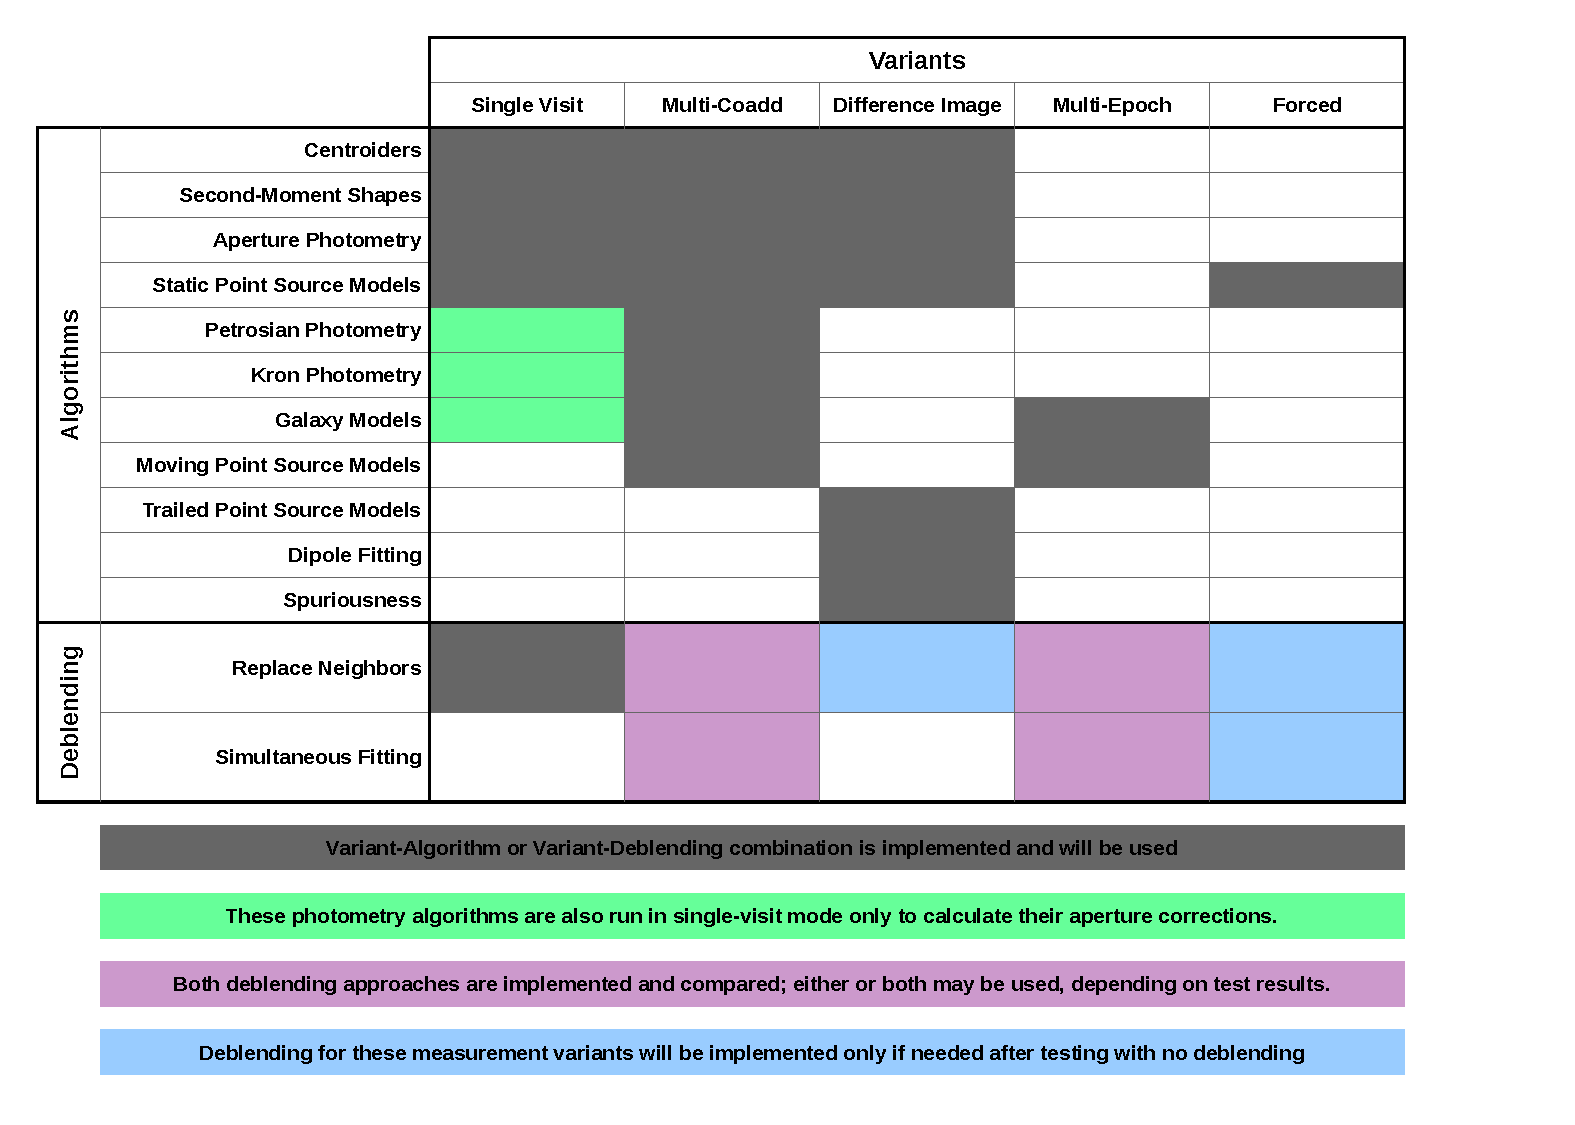
\includegraphics[width=\textwidth]{figures/measurement-matrix.pdf}
\caption{Matrix showing combinations of measurement variants, algorithms, and deblending approaches that will be implemented.
\label{fig:measurement-matrix}}
\end{figure}

\subsubsection{Drivers}
\label{sec:acMeasurementDrivers}
Measurement is run in several contexts, but always consists of running an ordered list of algorithm plugins on either individual objects or families thereof.  Each context corresponds to different variant of the measurement driver code, and has a different set of plugin algorithms and approaches to measuring blended objects.

\paragraph{Single Frame Measurement:} Measure a direct single-visit CCD image, assuming deblend information already exists and can be used to replace neighbors with noise (see \ref{sec:acReplaceNeighborsWithNoise}).
\label{sec:acSingleFrameMeasurement}

Single Frame Measurement is run in both \hyperref[sec:apSingleFrameProcessing]{AP's Single Frame Processing pipeline}) and DRP's \hyperref[sec:drpBootstrapImChar]{BootstrapImChar}, \hyperref[sec:drpRefineImChar]{RefineImChar}, and \hyperref[sec:drpFinalImChar]{FinalImChar}.

The driver for Single Frame Measurement is passed an input/output \hyperref[sec:spTablesSource]{SourceCatalog} and an \hyperref[sec:spImagesExposure]{Exposure} to measure.  Plugins take an input/output \hyperref[sec:spTablesSource]{SourceRecord} and an \hyperref[sec:spImagesExposure]{Exposure} containing only the object to be measured.

\paragraph{Multi-Coadd Measurement:} Simultaneously measure a suite of coadds representing different bandpasses, epoch ranges, and flavors.  This is run only in DRP's \hyperref[sec:drpMeasureCoadds]{MeasureCoadds} pipeline.
\label{sec:acMultiCoaddMeasurement}

The driver for Multi-Coadd Measurement is passed an input/output \hyperref[sec:spTablesObject]{ObjectCatalog} and a dict of \hyperref[sec:spImagesExposure]{Exposures} to be measured.  Plugins take an input/output \hyperref[sec:spTablesObject]{ObjectRecord} and a dict of \hyperref[sec:spImagesExposure]{Exposures}, each containing only the object to be measured.  Some plugins will also support simultanous measurement of multiple objects, which requires they be provided the subset of the \hyperref[sec:spTablesObject]{ObjectCatalog} to be measured and a dict of \hyperref[sec:spImagesExposure]{Exposures} containing just those objects.

\paragraph{Difference Image Measurement:} Measure a difference image, potentially using the associated direct image as well.  Difference image measurement is run in AP's \hyperref[sec:apAlertDetection]{Alert Detection} pipeline and DRP's \hyperref[sec:drpDiffIm]{DiffIm} pipeline.
\label{sec:acDiffImMeasurement}

The signatures of difference image measurement's drivers and algorithms are at least somewhat TBD; they will take at least a difference image \hyperref[sec:spImagesExposure]{Exposure} and a \hyperref[sec:spTablesSource]{SourceCatalog/SourceRecord}, but some plugins such as dipole measurement may require access to a direct image as well.  Because difference imaging dramatically reduces blending, difference image measurement may not require any approach to blended measurement (though any use of the associated direct image would require deblending).

If preconvolution is used to construct difference images, but they are not subsequently decorrelated, the algorithms run in difference image measurement cannot be implemented in the same way as those run in other measurement variants, and algorithms that cannot be expressed as a PSF-convolved model fit (such as second-moment shapes and all aperture fluxes) either cannot be implemented or require local decorrelation.

\paragraph{Multi-Epoch Measurement:} Measure multiple direct images simultaneously by fitting the same \hyperref[sec:spWCS]{WCS}-transformed, \hyperref[sec:spPSF]{PSF}-convolved model to them.  Blended objects in Multi-Epoch Measurement will be handled by \emph{at least} fitting them simutaneously (\ref{sec:acSimultaneousFitting}), which may in turn require hybrid galaxy/star models (\ref{sec:acHybridModels}).  These models may then be used as templates for deblending and replace-with-noise (\ref{sec:acReplaceNeighborsWithNoise}) measurement if this improves the results.
\label{sec:acMultiEpochMeasurement}

Because the memory and I/O requirements for multi-epoch measurement of a single object or blend family are substantial, we will not provide a driver that accepts an \hyperref[sec:spTablesObject]{ObjectCatalog} and measures all objects within it; instead, the \hyperref[sec:drpMultiFit] pipeline will submit individual family-level jobs directly to the orchestration layer.  The multi-epoch measurement driver will thus just operate on one blend family at a time, and manage blending while executing its plugin algorithms.

Multi-epoch measurement for DRP only includes two plugin algorithms, so it is tempting to simply hard-code these into the driver itself, but this driver will also need to support new plugins in Level 3.

Multi-epoch measurement will also be responsible for actually performing forced photometry on direct images, which it can do by holding non-amplitude parameters for moving point-source models fixed and adding a new amplitude parameter for each observation.

\paragraph{Forced Measurement:} Measure photometry on an image using positions and shapes from an existing catalog.
\label{sec:acForcedMeasurement}

In the baseline plan, we assume that forced measurement will only be run on difference images; while forced photometry on direct images will also be performed in DRP, this will be done in the course of multi-epoch measurement.

Because difference imaging reduces blending substantially, forced measurement may not require any special handling of blends.  If it does, simultaneous fitting (with point-source models) should be sufficient.

The driver for Forced Measurement is passed an input/output \hyperref[sec:spTablesSource]{SourceCatalog}, an additional input \hyperref[sec:spTablesReference]{ReferenceCatalog}, and an \hyperref[sec:spImagesExposure]{Exposure} to measure.  Plugins take an input/output \hyperref[sec:spTablesSource]{SourceRecord}, an input \hyperref[sec:spTablesReference]{ReferenceRecord} and an \hyperref[sec:spImagesExposure]{Exposure}.  If simultaneous fitting is needed to measure blends, plugins will instead receive subsets of the catalogs passed to the driver instead of individual records.

Forced measurement is used by the DRP \hyperref[sec:drpForcedPhotometry]{ForcedPhotometry} pipeline and numerous pipelines in AP.

\begin{note}[TODO]
Add references to specific AP pipelines that will use forced measurement.
\end{note}

\subsubsection{Algorithms}
\label{sec:acMeasurementAlgorithms}
\paragraph{Centroids}
\label{sec:acCentroidAlgorithms}

Centroid measurements are run on single images to measure the position of objects.  Despite the name, these don't measure just the raw centroid of the photons that correspond to an object; we generally also expect our centroid algorithms to correct for offsets introduced by convolution with the PSF.
While they may not be implemented this way, centroid algorithms should thus return results that are equivalent to the best-fit position parameters of a PSF-convolved symmetric model.  This model should be a delta function for unresolved objects and something approximately matched to the inferred size of extended objects.

When run in the very first stages of processing, a full PSF model will not be available, making PSF correction impossible, and here centroid measurements will be expected to yield the raw centroid of the light.  Note that this must still be corrected for any weighting function used by the algorithm.

Centroids will probably be run independently on each coadd during \hyperref[sec:acMultiCoaddMeasurement]{Multi-Coadd Measurement}, to allow for centroid shifts due to proper motion in short-period coadds.  Centroid measurements are superceded by \hyperref[sec:acMovingPointSourceModels]{Moving Point Source Models} and \hyperref[sec:acGalaxyModels]{Galaxy Models} in \hyperref[drpMultiFit]{MultiFit}, which impose different models for centroid differences between epochs that are consistent with morphology.  \hyperref[sec:ForcedMeasurement]{Forced Measurement} in production will never include centroid measurement, as the goal is explicitly to measure photometry at predetermined positions, but it may be useful to have the capability to centroid in forced measurement for diagnostic purposes.

\paragraph{Pixel Flag Aggregation}
\label{sec:acPixelFlags}

The pixel flag ``measurement algorithm'' simply computes summary statistics of masked pixels in the neighborhood of the source/object.  This provides a generic way to identify objects impacted by e.g. saturation or cosmic rays while allowing other measurement algorithms to ignore these problems (especially when they have been interpolated over.

\paragraph{Second-Moment Shapes}
\label{sec:acShapeAlgorithms}

Shape measurements here are defined as an estimate of a characteristic ellipse for a source or object that does \emph{not} attempt to correct for the effect of the PSF, corresponding to the second moments of its image.  To make this measurement practical in the presence of noise, a weight function must be used, and our baseline plan is to use an elliptical Gaussian matched (adaptively) to the shape of the image.  This may be unstable for sources with extremely low SNR, and for these the PSF, a fixed circular Gaussian, or a top-hat may be used as the weight function.  We may also include regularization that ensures the size of the object is no smaller than the size of the PSF.

To enable downstream code to correct shapes for the PSF, the shape algorithm must also measure the moments of the PSF model at the position of every object or source (though we expect the best PSF-corrected shape measures for galaxies to come from \hyperref[sec:acGalaxyModels]{Galaxy Model Fitting}).

\paragraph{Aperture Photometry}
\label{sec:acAperturePhotometry}

Aperture photometry here refers to fluxes measured within a sequence of fixed-size (i.e. same for all objects) circular or elliptical annuli.  The radii of the annuli will be logarithmically spaced radii, though fluxes at the largest largest radii will not be measured for objects significantly smaller than those radii.  Together these aperture fluxes will provide a measurement of the radial profile of the object.

The baseline plan for LSST is to use circular apertures, but we also plan to investigate using ellipses, which would provide more meaningful and higher SNR measurements if problems in robustly defining per-object (and perhaps per-radius) ellipses for faint objects can be solved.

While aperture fluxes with radii much larger than the pixel size can be measured naively by simply summing pixel values, smaller apertures will be measured using the $\mathrm{sinc}$ interpolation algorithm of \cite{2013MNRAS.431.1275B}, which integrates exactly over sub-pixel regions.  To avoid contamination from bleed trails when measuring heavily saturated objects, we plan to measure fluxes within azimuthal segments of annuli instead of circular regions; any the flux within any contaminated segments can be replaced by the mean of the remaining segments (thus assuming approximate circular symmetry).

For aperture fluxes with radii close to the PSF size to be scientifically useful, they must be performed on PSF-matched images.  We thus expect to plan run aperture photometry only on PSF-matched coadds and visit-level images, with the latter accompanied by a caution that smaller apertures may not be meaningful without user-level correction for the PSF.

\paragraph{Static Point Source Photometry}
\label{sec:acStaticPointSourceModels}

In single-visit, difference image, and forced measurement, PSF fluxes will be measured with position held fixed at the valued determined by the \hyperref[ac:CentroidAlgorithms]{Centroid algorithm}, with only the amplitude allowed to vary.  We will not use per-pixel weights (as these can lead to bias as a function of magnitude when the PSF model is slightly incorrect) to fit for the amplitude, but we will use per-pixel variances to compute the uncertainty on the flux.  PSF fluxes will be aperture corrected (see Section~\ref{sec:acApCorr}).

In multi-coadd measurement we may use either static point source models or moving point source models to estimate PSF fluxes; this depends on the number and depth of short-period coadds, and hence it is likely we will use static point source models for early data releases and moving point source models near the end of the survey.  In either case we expect these measurements to be entirely superceded for science purposes by multi-epoch fitting results using a moving point-source model; these measurements on coadds are largely for QA and to warm-start multi-epoch fitting.

\paragraph{Kron Photometry}
\label{sec:acKronPhotometry}

Kron fluxes are aperture fluxes measured with an aperture radius set to some multiple (usually $2$ or $2.5$) of the Kron radius, which is defined as:

$$
R_{\mathrm{kron}} = \frac{\sum r \, I(r)}{\sum I(r)}
$$

In our implementation, we use an elliptical aperture (and compute the above radius using elliptical moments), using the \hyperref[sec:acShapeAlgorithms]{Second-Moment Shape} to set the ellipticity.

Measuring the Kron radius itself is difficult in the presence of noise; as with any moment measurement, pixels far from the center with low SNR are given higher weight than central pixels with high SNR.  In practice, the sums over pixels in the Kron radius definition must be truncated at some point, and the resulting Kron radius can be sensitive to this choice.  Our current approach uses a fixed multiple of the \hyperref[sec:acShapeAlgorithms]{Second-Moment Shape} ellipse.  This may be less robust than an adaptive approach, but it more closely matches the procedure used by SExtractor's \texttt{MAG\_AUTO}, which is by far the most popular implementation of Kron photometry in astronomy.


\paragraph{Petrosian Photometry}
\label{sec:acPetrosianPhotometry}

\begin{note}
Need to get RHL to write this section.
\end{note}

\begin{itemize}
\item Compute Petrosian radius.
\item Requires taut splines and more robust measurement of standard elliptical aperture suite.
\item Compute flux in elliptical aperture at multiple Petrosian radius.
\end{itemize}


\paragraph{Galaxy Models}
\label{sec:acGalaxyModels}

Galaxy models will be fit to all objects in both \hyperref[sec:acMultiEpochMeasurement]{Multi-Epoch Measurement} and \hyperref[sec:acMultiCoaddMeasurement]{Multi-Coadd Measurement}.  Coadd fitting may be performed only on deep coadds and used to warm-start multi-epoch fitting that would supersede it, but it may also be run on PSF-matched coadds to generate consistent colors (the consistent colors referred to by the \DPDD{} may be derived from galaxy models fit to PSF-matched coadds or aperture fluxes on PSF-matched coadds, but they may also be derived from multi-epoch fitting results).

The baseline plane for the galaxy models themselves is a restricted bulge + disk model, in which the two components are restricted to the same ellipticity and the ratio of their radii is fixed; practically this is more analogous to a single Sersic model with a linearized Sersic index.  This may be extended to models with more flexible profiles and/or different ellipticity and radii for the two components if these additional degrees of freedom can still be fit robustly.  Bayesian priors and possibly other regularization methods will likely be necessary even with the baseline degrees of freedom.

Designing and constraining priors that provide the right amount of information in the right way is a major challenge.  One possibility is an empirical prior derived from external datasets such as deep HST fields and precursor ground-based surveys, which would almost certainly require custom processing of those datasets using the models intended for production use.  Hierarchical modeling -- in which the prior is derived from the LSST wide survey itself as individual objects are fit -- is unlikely to be feasible (a naive implementation would either introduce \emph{several} full-survey, all-object sequence points in the processing or treat galaxies processed late differently from those processed early).  An empirical prior derived from LSST special program data (e.g. deep drilling fields) or previous data releases would be feasible, however, and should be considered.  Even an ideal prior that reflects the true distribution of galaxy parameters may not be appropriate for galaxy photometry, however; fluxes must be rigorously defined to be unbiased to changes in observing conditions, and are most useful when they can be defined in a way that is redshift-independent as well.  The ``correct'' Bayesian prior \emph{explicitly} treats galaxies with different radii differently, making both of these properties harder to guarantee.  As a result, the prior we use for fitting may be some compromise between the statistically appropriate distribution and a regularization that attempts to reconcise Bayesian modeling with the requirements of traditional maximum-likelihood photometry.

In addition to maximum-posterior fitting, we will draw Monte Carlo samples (nominally 200 samples per object, at least on average) from the posterior in multi-epoch fitting mode.  Fitting this within LSST's computational budget will be a serious challenge, requiring new algorithm development in several areas:
\begin{itemize}
\item Evaluating PSF-convolved galaxy models on every epoch at every sample point or optimizer iteration is extremely expensive.  Because galaxy models are generally massively undersampled before convolution with the pixel grid, naive pixel convolution is impossible without considerable subsampling, which genreally makes it computationally impractal.  Fourier-space methods require galaxy models with anayltic Fourier transforms as well as a great deal of care in accounting for the differences between discrete and continuous Fourier transforms.  Multi-Gaussian and Multi-Shapelet approximation methods are only computationally feasible if the PSF can consistently be approximated well by those functions, which may not be known until relatively late in commissioning.  It may be possible to combine the multi-Gaussian and Fourier-space convolution approaches by using multi-Gaussian approximations to galaxy models to evaluate them efficiently in Fourier space.  We may also be able to address large residuals from multi-Gaussian/multi-Shapelet PSF approximations by convolving the residuals themselves with a simple proxy for the galaxy model (which could be a delta function for small galaxies) and adding this as a correction to the multi-Gaussian/multi-Shapelet convolution.
\item Most Monte Carlo methods require many more than 200 draws to converge to a fair sample (for galaxy-fitting problems, $\sim 10^4$ is common).  We plan to use importance sampling in multi-epoch fitting, starting with samples drawn from the posterior distribution in coadd-fitting (where we can evaluate likelihoods faster by a factor of the number of exposures in each band on average).  These samples must be self-normalized, which introduces a bias that may be significant if the number of samples is small, and it is currently unclear whether this will be a problem in our case.  It is also unlikely we will be able to draw as many as $\sim 10^4$ samples even in coadd measurement in order to achieve convergence there.  Results from fitting with a greedy optimizer first should provide enough information allow for fair and efficient sampling with a smaller number of draws, but devising a sampling algorithm to make use of that information may be challenging.
\end{itemize}

Challenges in galaxy modeling are not limited to sampling; the effective number of galaxy model evaluations involved in a typical greedy optimizer fit is also at least 200, if evaluations needed to estimate derivatives via finite differences are included (and analytic derivates are usually not significantly faster than numerical derivatives).  Galaxy model parameterizations are intrinsically difficult for most optimizers near the zero radius limit, as this forces the derivative of the model with respect to other parameters (such as ellipticity) to approach zero as well.  Issues with Bayesian priors causing flux biases and the general lack of sufficient information to constrain more complex models are also present for optimizer-based fitting.  Priors are perhaps a larger concern for fitting than sampling, in fact, because users can reweight samples to replace a DM-selected prior with a prior of their own choosing, but this is only approximately possible for optimizer results.

Galaxy models may be fit simultaneously to multiple objects (see \hyperref[sec:acSimultaneousFitting]{Simultaneous Fitting}) as well as fit to individual objects after \hyperref[sec:acReplaceNeighborsWithNoise]{replacing neighbors with noise}.  In simultaneous fitting, it will sometimes be inappropriate to fit all objects in a blend with galaxy models.  Fitting \hyperref[sec:acHybridModels]{Hybrid Models} that can transition smoothly between a galaxy model and a \hyperref[sec:acMovingPointSourceModels]{Moving Point Source Model} is one approach to avoid fitting all permutations of model types to a blend.

\begin{note}[TODO]
Cite Lensfit paper for restricted bulge-disk model.  Cite Hogg and Lang, Bosch 2010 for Gaussian/Shapelet approximation.
\end{note}

\paragraph{Moving Point Source Models}
\label{sec:acMovingPointSourceModels}

In the \hyperref[sec:acMultiEpochMeasurement]{Multi-Epoch Measurement}, all objects will be fit with a moving point source model that includes proper motion and parallax as free parameters in addition to positional zeropoint and per-band amplitudes.  This model may be extended to include parameterized variability or per-epoch amplitudes if this can be done without degrading the astrometric information that can be extracted from the fit.  Moving point source models may be fit in \hyperref[sec:acMultiCoaddMeasurement]{Multi-Coadd Measurement} as well if the suite of coadds contains enough short-period coadds to constrain the fit, but these results will be fully superseded by the \hyperref[sec:acMultiEpochMeasurement]{Multi-Epoch Measurement} results.

Bayesian priors may be used in the fit (making this ``maximum posterior'' instead of ``maximum likelihood''), if necessary to ensure robustness when fitting for faint objects or if they significantly improve the quality of the results.   These will generally be global and relatively uninformative (reflecting e.g. the expected distribution of proper motion of stars as a function of apparent magnitude), but may be highly informative for stars that can be unambiguously associated with the Gaia catalog, if including Gaia and LSST astrometric solutions at the catalog level proves inconsistent with this (more rigorous) Bayesian approach to including Gaia data at the pixel level.  All priors will be reported, but unlike Monte Carlo samples, results from a fit with a greedy optimizer cannot be reweighted to change to a user-provided prior except in a perturbative, first-order sense.  Monte Carlo sampling with moving point source models is not included in the baseline plan, but will be considered if it proves important for joint fitting of blended stars and galaxies (see \hyperref[sec:acHybridModels]{Hybrid Models}, below) or \hyperref[sec:acObjectClassification]{Star/Galaxy Classification}, and it can be done without significantly affecting the compute budget.

\begin{note}[TODO]
Cite Lang+Hogg paper that did this in Stripe 82.
\end{note}

\paragraph{Trailed Point Source Models}
\label{sec:acTrailedPointSourceModels}

\begin{note}
Need to find someone (probably on AP team) to write this section.
\end{note}

\begin{itemize}
\item Fit PSF convolved with line segment to individual images
\end{itemize}

\paragraph{Dipole Models}
\label{sec:acDipoleModels}
\begin{itemize}
\item Fit PSF dipole for separation and flux to a combination of difference image and direct image.
\item Deblending on direct image very problematic.
\end{itemize}

Arising primarily due to slight astrometric alignment or PSF matching errors between the two images, or effects such as differential chromatic aberration, flux “dipoles” are a common artifact often observed in image differences. These dipoles will lead to false detections of transients unless correctly identified and eliminated. Importantly, dipoles will also be observed in image differences in which a source has moved less than the width of the PSF. Such objects must be correctly identified and measured as dipoles in order to obtain accurate fluxes and positions of these objects.

Putative dipoles in image differences are identified as a positive and negative source whose footprints overlap by at least one pixel. These overlapping footprints are merged, and only the sources containing one and only one positive and negative merged footprint are passed to the dipole modeling task. There is a documented degeneracy \citedsp{DMTN-007} between dipole separation and flux, such that dipoles with closely-separated lobes of high flux are statistically indistinguishable from ones with low flux and wider separations. We remove this degeneracy by using the \emph{pre-subtraction images} (i.e., the warped, PSF-matched template image and the pre-convolved science image) to constrain the lobe positions (specifically, to constrain the centroid of the positive lobe in the science image and of the negative lobe in the template image). This is done by first fitting and subtracting a second-order 2-D polynomial to the background within a subimage surrounding each lobe footprint in the pre-subtraction images to remove any flux from background galaxies (we assume that this gradient, if it exists, is identical in both pre-subtraction images). Then, a dipole model is fit simultaneously to the background-subtracted pre-subtraction images and the image difference.

The dipole model consists of positive and negative instances of the PSF in the difference image at the dipole's location. The six dipole model parameters (positive and negative lobe centroids and fluxes) are estimated using non-linear weighted least-squares minimization (we currently use the Levenberg-Marquardt minimization algorithm). The resulting reduced $\chi^2$ and signal-to-noise estimates provide a measure by which the source(s) may be classified as a dipole.

We have tested the described dipole measurement algorithm on simulated dipoles with a variety of fluxes, separations, background gradients, and signal-to-noise. Including the pre-subtraction image data clearly improves the accuracy of the measured fluxes and centroids. We have yet to thoroughly assess the dipole measurement algorithm performance on crowded stellar fields. Such crowded fields may confuse the parameter estimates (both centroids and/or fluxes) when using the pre-subtraction images to constrain the fitting procedure, and in such situations, we may have to adjust the prior constraint which they impose.

Note that deblending dipole sources is a complicated process and we do not intend on implementing such an algorithm.  As with all fitting algorithms, speed may be a concern.  We will optimize the dipole measurement for speed.

\paragraph{Spuriousness}
\label{sec:acSpuriousnessAlgorithms}

\begin{note}
Need to find someone (probably on AP team) to write this section.
\end{note}

\begin{itemize}
\item Some per-source measure of likelhood the detection is junk (in a difference image).
\item May use machine learning on other measurements or pixels.
\item May be augmented by spuriouness measures that aren't purely per-source.
\end{itemize}

\subsubsection{Blended Measurement}
\label{sec:acBlendedMeasurement}

Most LSST objects will overlap one or more of its neighbors enough to affect naive measurements of their properties.  One of the major challenges in the deep processing pipelines will be measuring these objects in a way that corrects for and/or characterizes the effect of these blends.

The measurement algorithms of Section~\ref{sec:acMeasurementAlgorithms} can be split up broadly into two categories:
\begin{itemize}
    \item weighted moments (includes \hyperref[sec:acShapeAlgorithms]{Second-Moment Shapes}, \hyperref[sec:acAperturePhotometry]{Aperture Photometry}, \hyperref[sec:acKronPhotometry]{Kron Photometry}, and \hyperref[sec:acPetrosianPhotometry]{PetrosianPhotometry};
    \item forward modeling (includes \hyperref[sec:acGalaxyModels]{Galaxy Models}, \hyperref[sec:acMovingPointSourceModels]{Moving Point Source Models}, and \hyperref[sec:acTrailedPointSourceModels]{Trailed Point Source Models}).
\end{itemize}

Most measurements that involve the PSF or a PSF-convolved function as a weight function can be interpreted in either way (this includes most \hyperref[sec:acCentroidAlgorithms]{Centroid} algorithms and all PSF flux algorithms), though only the weighted-moment interpretation provides a motivation for ignoring per-pixel variances, as is necessary to ensure unbiased fluxes in the presence of incorrect models.

The statistical framework in which weighted moments make sense assumes that each object is isolated from its neighbors.  As a result, our only option for these measurements is removing neighbors from the pixel values prior to measurement, which we will discuss further in \ref{sec:acReplaceNeighborsWithNoise}.

In forward modeling, we convolve a model for the object with our model for the PSF, compare this model to the data, and either optimize to find best-fit parameters or explore the full likelihood surface in another way (e.g. Monte Carlo sampling).  We can use the removing-neighbors approach for forward fitting, simply by fittting each object separately to the deblended pixels.  However, we can also use simultaneous fitting (Section~\ref{sec:acSimultaneousFitting}), in which we optimize or sample the models for multiple objects jointly.

Both neighbor-replacement and simultaneous fitting have some advantages and disadvantages:
\begin{itemize}
\item Neighbor-replacement provides no direct way to characterize the uncertainties in an object's measurements due to neighbors, while these are naturally captured in the full likelihood distribution of a simultaneous fit.  This likelihood distribution may be very high-dimensional in a fit that involves many objects, however, and may be difficult to characterize or store.
\item Neighbor-replacement generally allows for more flexible morphologies than the analytic models typically used in forward fitting, which is particularly important for nearby galaxies and objects blended with them; simultaneous fitting is only statistically well-motivated to the extent the models used can reproduce the data.
\item Once neighbor-free pixels are available, fitting objects simultaneously will almost always be more computationally expensive than fitting them separately to the deblended pixels.  At best, simultaneous fitting will have similar performance but still require more complex code.  And because we will need to deblend pixels to support some measurement algorithms, we'll always have to deblend whether we want to subsequently do simultaneous fitting or not.
\end{itemize}

\paragraph{Neighbor Noise Replacement}
\label{sec:acReplaceNeighborsWithNoise}

We do not perform measurements directly on the deblended-pixel \hyperref[sec:spFootprintsHeavy]{HeavyFootprints} output by the \hyperref[sec:acDeblending]{Deblender} for two reasons:
\begin{itemize}
\item The deblended pixels typically have many zero entries, especially for large blend families (i.e. many pixels for which a particular object has no contribution).  These zero pixels make the noise properties of a deblended object qualitatively different from those of an isolated object, which may be problematic for some measurement algorithms.
\item Many measurements utilize pixels beyond the blend family's \hyperref[sec:spFootprintsHeavy]{Footprint}, and in fact may extend to pixels that are in another family.
\end{itemize}
To address these issues, we measure deblended objects using the following
procedure:
\begin{enumerate}
\item Replace every above threshold pixel in the image (all \hyperref[sec:spFootprints]{Footprints}) with randomly generated noise that matches the background noise in the image.
\item For each blend family:
    \begin{enumerate}
    \item For each child object in the current blend family:
        \begin{enumerate}
        \item Insert the child's \hyperref[sec:spFootprintsHeavy]{HeavyFootprint} into the image, replacing (not adding to) any pixels it covers.
        \item Run all measurement algorithms to produce \emph{child} measurements.
        \item Replace the pixels in the child's \hyperref[sec:spFootprints]{Footprint} region with (the same) random noise again.
        \end{enumerate}
    \item Revert the pixels in the parent \hyperref[sec:spFootprints]{Footprint} to their original values.
    \item Run all measurement algorithms to produce \emph{parent} measurements.
    \item Replace the parent \hyperref[sec:spFootprints]{Footprint} pixels with (the same) random noise again.
    \end{enumerate}
\end{enumerate}
This procedure double-counts flux that is not part of a \hyperref[sec:spFootprints]{Footprint}, but this is considered better than ignoring this flux, because most measurement algorithms utilize some other procedure for downweighting the contribution of more distant pixels.

\paragraph{Deblend Template Projection}
\label{sec:acDeblendTemplateProjection}

When \hyperref[sec:acDeblending]{deblending} is performed on one image and measurement occurs in another, the deblender outputs must be ``projected'' to the measurement image.  In general, this requires accounting for three potential categories of differences between the images:
\begin{itemize}
\item differing coordinate systems
\item differing PSFs
\item different epoch.
\end{itemize}
We do not currently have a use case for projecting deblender results between images with different filters; we expect that we will have deblender results from at least each per-band coadd, and projection is required for different per-epoch images in \hyperref[sec:acForcedMeasurement]{Forced Measurement} and \hyperref[sec:acMultiEpochMeasurement]{Multi-Epoch Measurement}.  It may be entirely unnecessary if \hyperref[sec:acSimultaneousFitting]{Simultaneous Fitting} can be used to address all blended measurement issues in these contexts.

When variability can be ignored, deblended pixel values can be \hyperref[sec:spWarp]{resampled} using the same algorithms that operate on images, and \hyperref[sec:acPsfMatching]{PSF Matching} kernels can be used to account for PSF differences (though some regularization will be required if this involves a deconvolution).  When variability cannot be ignored, these operations should instead be applied to the deblend templates, which can then be re-fit to produce new per-epoch deblend results.

These operations are significantly easier if the deblend templates themselves are defined via analytic models that must be convolved with the PSF to generate the template; the models can simply be transformed, convolved with the per-epoch PSF and re-fit.

\paragraph{Simultaneous Fitting}
\label{sec:acSimultaneousFitting}

For measurement algorithms that can be fully expressed as a likelihood-based fit using a model that closely approximates the data, an alternative to \hyperref[sec:acReplaceNeighborsWithNoise]{Neighbor Noise Replacement} is to fit all objects in a blend simultaneously (either with a greedy optimizer or with Monte Carlo sampling).  This is statistically straightforward: the parameter vectors for individual per-object models can simply be concatenated, and the pixels to fit to are the union of all of the pixels that would be used in fitting individual objects.

Simultaneously fitting a group of objects is almost certainly slower than fitting those objects individually, in essentially every case, but the decrease in performance may be mild.  The per-iteration calculations in optimizer-based methods have a worst-case complexity that is $O(N^2)$ in the number of parameters, but the $O(N)$ evaluation (and convolution) of models typically completely dominates the $O(N^2)$ linear algebra, and this should hold for all but the very largest blend families.  The more important scaling factor is the number of iterations required to converge to the solution; as this is expected to scale roughly with the volume of the space that much be searched, it could scale as poorly as $O(k^N)$.  This can be ameliorated by starting the optimizer close to the correct solution; fitting objects independently to deblended pixel values before simultaneous fitting should provide a reasonably good guess.  Simultaneous fitting in \hyperref[sec:acMultiEpochMeasurement]{Multi-Epoch Measurement} can also be initialized from the results of \hyperref[sec:acMultiCoaddMeasurement]{Multi-Coadd Measurement}, where model evaluations are significantly faster.

With Monte Carlo methods, a high-dimensional parameter space is less of a problem; Monte Carlo methods are valued precisely because they scale (on average) better with dimensionality.  We still expect to require warm-start methods for simultaneous Monte Carlo sampling of multiple objects, such as using importance sampling in \hyperref[sec:acMultiEpochMeasurement]{Multi-Epoch Measurement} to re-weight samples drawn during independent per-object sampling or \hyperref[sec:acMultiCoaddMeasurement]{Multi-Coadd Measurement}.

For both optimizer-based fitting and Monte Carlo sampling, it should be possible to explore the parameter space in a way that does not require evaluating the model for every object at every iteration or draw; because objects on opposite sides of a blend should affect each other only weakly, optimizer steps and samples that explicitly ignore these weak correlations in choosing the next parameter point to evaluate may be more efficient.  In Monte Carlo sampling, this would probably utilize techniques from Gibbs Sampling; with optimizers, one can probably ignore the step for any objects whose optimal step size falls below some threshold (with some extra logic to guarantee these objects are are still sometimes updated).  These improvements would likely reuqire significant development effort, and they would almost certainly make using off-the-sheld optimizers and samplers impossible.

The fact that simultaneous fitting itself may be used to produce templates for deblending -- and that simultaneous fitting may require non-simultaneous fitting, using deblended results, for a warm start -- suggests that the boundary between the \hyperref[sec:acDeblending]{Deblending} and measurement algorithmic components may be somewhat vague.  This could be represented in software as an iteration between these algorithmic components, or perhaps a hierarchy of components in which the same low-level fitting code is used (and extended) by both algorithmic components, which can then be run straightforwardly in sequence.

\paragraph{Hybrid Models}
\label{sec:acHybridModels}

In simultaneous fitting, the model used to fit one object can affect the quality of the fit to its neighbor, making it important the the best model be used for each object.  We explicitly fit both \hyperref[sec:acMovingPointSourceModels]{Moving Point Source Models} and \hyperref[sec:acGalaxyModels]{Galaxy Models} to every object, however, precisely because we do not expect to always be able to securely classify objects well enough to know which model is better (and we certainly do not expect to be able to classify them before fitting these models).  In simultaneous fitting, trying all possibilies leads to a combinatorial explosion of model-fitting jobs (fitting each of two models to $N$ objects leads to $2^N$ fits).

Given that both of these models have a static point source as a limit, and classification is hardest at this limit, making the right classification for neighbors may not be critical; misclassified objects would still end up being fit with a model that is broadly appropriate for them.  Even in this case, we would still have $2N$ fitting objects when fitting an $N$-object blend with two models: every object would be fit twice as the ``primary'' object (with both models), and then twice for each of its neighbors.  Given that each of these fitting jobs still involves fitting $N$ objects, this still results in a scaling of approximately $2N^2$ (clever optimizers and samplers could probably reduce this, with a cost in code complexity and development time).

Another option would be to fit both models simultaneously, by introducing a higher-level boolean parameter that sets the type.  Sampling from this hierarchical model is not significantly difficult than sampling from either of the original models if naive samplers are used, but optimizers and samplers that rely on derivative information will likely have trouble dealing with the discrete type parameter.  It may be possible to define a smooth transition between the two models through the static point source limit they share, though this would likely require customization of the optimizer and sampler as well.  Sampling with this sort of hybrid model would naturally produce samples from both models in the proportion weighted by the marginal probability of those models, which is essentially ideal (assuming sampling is considered useful for \hyperref[sec:acMovingPointSourceModels]{Moving Point Source Models}).  Using an optimizer with hybrid models would result in a result for just the best-fit model, which is somewhat less desirable.

\subsection{Spatial Models}
\label{sec:acSpatialModels}
In many areas we will need to represent spatial models (generally over CCDs, visits, or coadd patches).  PSF models, sky backgrounds, aperture corrections, and WCSs all involve spatial variation on these scales, and at least some of these should share lower-level algorithm code to fit the spatila models.  This will include models fit to sparse and non-uniformly sampled data.  We will support fitting Chebyshev polynomials and splines.  We will also support regression techniques like Gaussian Processes.

\subsection{Background Estimation}
\label{sec:acBackgroundEstimation}

\subsubsection{Single-Visit Background Estimation}
\label{sec:acSingleVisitBackgroundEstimation}

Background estimation will be done on the largest scale feasible first.  In the case of Alert Production, this may be on the size of a chip.  In DRP, we expect this to be on a full focalplane.  An initial low order estimate will be made on a large scale.  Each chip will be divided into subregions.  For each subregion, a robust average of the non-masked pixels will be computed.  All values for all chips will be fit by an appropriate function (see \S \ref{sec:acSpatialModels}).  This will provide a low order background estimation in focal plance coordinates.  Note that this can only be done if the Instrument Signature Removal is very high fidelity.  Any sharp discontinuity could cause problems with fitting a smooth function.

A higher order background model can be computed per chip.  First, the low order background is subtracted from the image.  The non-masked pixels will again be binned on a finer grid avoiding bright objects.  The median in each bin is fit by an appropriate function.  In practice, this process will likely be iterative.

In the case of Alert Production, there will be no full focalplane model since we expect to process only a single chip in each thread.  In this case, we constrain the background with the available un-masked pixels without removing a global background first.  Note that image differencing is still possible even in the scenario where there are no unmasked pixels in the science image.  The background can be modeled as a part of the PSF matching process.  We will want to do background modeling and subtraction in Alert Production when possible because we will want to do calibrated photometry.  Even though these measurements are not persisted for science use, they will be very useful for debugging and QA.

If there are so few un-masked pixels in the entire focalplane that even a low order global background is impossible to model, background modeling may need to be iterated with a procedure that models and subtracts stars (for example, see the \hyperref[sec:drpBootstrapImChar]{BootstrapImChar pipeline in DRP}).

\begin{note}[Crowded fields and composition]
Requirements include working in crowded fields.  I think estimating a full focalplane model is the best we can do.  If there are no unmasked pixels in the entire FoV, I don't think there is much we can do.
I didn't explicitly talk about composition of background models, but this takes that into account by allowing a global model to be subtracted from the single chip image before a higher order model is fit.
\end{note}

\subsubsection{Coadd Background Estimation}
\label{sec:acCoaddBackgroundEstimation}

A variant of \hyperref[sec:acSingleVisitBackgroundEstimation]{Single-Visit Background Estimation} that is run on coadds to model the remaining background that is not removed during background matching.  This includes the observational background from the reference image

\subsubsection{Matched Background Estimation}
\label{sec:acMatchedBackgroundEstimation}

A variant of \hyperref[sec:acSingleVisitBackgroundEstimation]{Single-Visit Background Estimation} for use on difference images produced in \hyperref[sec:drpBackgroundMatchAndReject]{Background Matching}.  This will be able to operate on full visit scales with much less concern for oversubtracting bright objects, which may allow it to use qualitatively different algorithms.  It may also be able to use models specifically designed to subtract specific ghosts or stray light patterns.

\subsection{Build Background Reference}
\label{sec:acBuildBackgroundReference}
% AUTHOR: Simon

\subsubsection{Patch Level}
Background-matching each \texttt{CoaddTempExp} to a reference exposure performs comparably to fitting
the offsets to the N(N-1)/2 difference images, however the co-add quality will depend on the quality of the
reference image.  Choosing a reference image on a per-patch basis is as simple as choosing the \texttt{CoaddTempExp} that
maximizes coverage and is the highest weighted component in the chosen weighting scheme: e.g. minimum variance, optimum point source SNR.

Coverage is defined as the fraction of non-NaN
pixels in the \texttt{CoaddTempExp}. NaN pixels arise in \texttt{CoaddTempExp}s because of gaps between the chips and edges of the visit focal
planes.  The camera design specifications indicate a 90\% fill factor, and thus approximately 10\% of pixels
will be NaN due to chip gaps.  The SNR of the background can be estimated from either the \texttt{CoaddTempExp}s themselves,
using the variance plane of pixels without the source detection bit mask flagged, or from calibration
statistics such as the zero point (a proxy for transparency).  In the limiting case that all \texttt{CoaddTempExp}s have the
same coverage, finding the best reference image reduces to the problem of weighting epochs in co-addition.

For example, the reference image that minimizes the variance in the co-add is the minimum variance \texttt{CoaddTempExp}, and
the reference image that maximizes SNR in coadd point source measurements is the \texttt{CoaddTempExp} with the maximum
$T^2_i/\mathrm{FWHM}^2_i \sigma^2_i$, where $T_i$ is
the normalization factor necessary to put the input \texttt{CoaddTempExp}s on the same photometric system (a proxy for the atmospheric transparency),
and $\sigma^2_i$ the average variance of the pre-scaled exposure.  By combining one of
these statistics with coverage, we can construct an objective/cost function that relates the importance of
coverage and sky-background, and can select a visit that minimizes that quantity objective function.

\subsubsection{Tract Level}
Constructing reference images for tract-sized co-adds follows the same principle, but requires maximizing the
SNR/coverage of a large mosaic constructed from multiple visits.  Algorithms for mosaicking partially
overlapping images have been well established \citep[e.g.][]{2014AJ....147..109S, 2008ASPC..394...83B}. By mosaicking visits,
applying additive scalar or sloping offsets to calexps, we can generate a tract-sized reference image.
Algorithms for selecting visits to construct these fall on a spectrum of computational expense. On the less
expensive side is a greedy algorithm which starts with a ``best'' (as defined above) visit chosen at the
center of the tract.  Visits can be chosen, scaled, and added one by one in the vicinity, moving outwards.
Another option is to choose a small set of visits that completely cover a tract without gaps, which can b
cast as a constrained convex optimization problem\footnote{probably}, and mosaic them using standard
mosaicking techniques.  Finally, the most expensive option would use all the visits to simultaneously tie the
visits together using all overlaps while background matching.

\subsection{PSF Estimation}
\label{sec:acPSFEstimation}

\subsubsection{Single CCD PSF Estimation}
\label{sec:acSingleCCDPSF}

Single CCD PSF estimation needs to be run in both Alert Production and in Data Release Processing.  In Alert Production it will be the final PSF model for both direct and difference image measurement.  In Data Release Processing, it will be used as an initial bootstrapping step to start off image characterization.  We do not expect to require inclusion of chromatic effects in the PSF at the single CCD estimation phase.

The first step is to select a set of suitable stars to use as PSF exemplars.  In production, we expect that an external catalog with PSF candidates that have been shown to be non-varying and isolated will produce the most repeatable results.

Once a set of candidate stars is selected each star is fit by a set of
appropriate basis functions (e.g., PCA or pixel bases).  The PSF is approximated by
\[
P = \Sigma_n c_n\Psi_n
\]
where $\Psi_n$ is the $n^{th}$ basis function, and $c_n$ is the coefficient for that basis function.  We can solve for the coefficients for each PSF candidate in a least squares sense along with a model for the spatial variation of the PSF
across the CCD.

\begin{note}{JFB}
    This algorithm is unlikely to work in crowded fields, where are no
    isolated stars and hence it will probably be impossible to perform a PCA
    of star images, and there's no way to separate kernel image fitting from
    spatial interpolation.  If fitting a PSF in crowded fields is necessary
    (for some image differencing algorithms, building image differencing
    templates, or the stretch goal of performing crowded-field photometry),
    we should consider starting with something simple, like a double-Gaussian
    and iteratively running a traditional (Alard-Lupton-style) image-
    differencing code between the science image and the model image to
    generate an update to the PSF model (this is RHL's idea; I'm just stating
    it).
\end{note}

\subsubsection{Wavefront Sensor PSF Estimation}
\label{sec:acWavefrontSensorPSF}
%AUTHOR: Jim
\begin{itemize}
\item Build an approximate PSF model using only the very brightest stars in the wavefront sensors.  Because WF sensors are out-of-focus, these stars may be saturated on science CCDs.
\item Model can have very few degrees of freedom (very simple optical model + elliptical Moffat/Double-Gaussian?)
\item Only needs to be good enough to bootstrap PSF model well enough to bootstrap processing of science images (but it needs to work in crowded fields, too).
\item Being able to go to brighter magnitudes may be important in crowded fields because the shape of the luminosity function may make it easier to find stars with (relatively) significant neighbors.
\item Assumed to be at least mostly contributed by Telescope and Site.
\end{itemize}

\subsubsection{Full Visit PSF Estimation}
\label{sec:acFullVisitPSF}

This algorithm represents our most careful and computationally expensive PSF estimation algorithm, and will be run only in DRP.  We anticipate a model that decomposes the PSF into components for the optical system and the atmosphere.  This should improve our ability to interpolate between star positions, provide physically-motivated wavelength dependence, and a way to interpolate the PSF model between CCDs.

The optical component will be modeled in wavefront space using Zernike polynomials, but we will not use Zernike polynomial coefficients directly; instead, we will use an exploration of out-of-focus images to develop a model that relates the physical degrees of freedom (or some empirical-determined estimate of these) to the changes in the wavefront across the focal plane, and use those degrees of freedom as the free parameters in the optical model.

The model for the atmospheric componet is less clear.  A simple elliptical model with a standard (Moffat, Kolmogorov, multi-Gaussian) profile may be adequate, with ellipticity and size interpolated using Gaussian processes.  If not, we will consider using such a model as a starting point from which we can iteratively fit a pixel-based (or other similarly flexible) model with the optical model; a major concern is that a too-flexible model will be degenerate with the optical model.

The parameters of both components will be fit either iteratively or simultaneously to the images of a set of secure stars across the entire focal plane.  Images of out-of-focus stars from wavefront sensors may be utilized as well, but it is not clear yet how helpful they will be.

In addition to using the above techniques to model the core of PSF, this algorithm is also responsible for estimating the wings of the PSF for bright stars, which may use entirely different (likely fully empirical) techniques.

\subsection{Aperture Correction}
\label{sec:acApCorr}

While photometric calibration is responsible for ensuring that one measure of flux is defined consistently both across epochs and with external datasets, aperture corrections are responsible for ensuring internal consistency between different flux measures.

Aperture corrections for stars are straightforward but difficult in practice:
\begin{itemize}
\item Using a sequence of fixed-aperture fluxes from a sample of secure bright stars in a visit, we model the curve of growth as a (weak) function of position on the focal plane.  This may involve utilizing measurements from saturated stars to improve the signal-to-noise ratio in the largest apertures.
\item Given this model, define the aperture correction for a photometry algorithm as the spatially-varying ratio of the extrapolated curve-of-growth flux to the flux measured by that algorithm (on the same sample of stars); like the curve-of-growth model, these aperture corrections are modeled as a weak function of position on the focal plane.
\end{itemize}
This scheme naturally puts the sequence of fixed-radius aperture fluxes on the same photometric system as the aperture-corrected fluxes if they are considered as a radial profile (i.e. they approach the total flux as the radius increases).  We may also want to aperture-correct some fixed-radius aperture fluxes so they too reflect the total flux.

The uncertainty in estimating aperture corrections should be estimated and propagated to the corrected fluxes.  This is tricky, because the sequence of aperture fluxes use many of the same pixels for each as the algorithm we are tying to them, making them their uncertainties highly correlated.  To address this, all aperture-corrected photometry algorithms will have to be able to report the pixels they use in a measurement to allow this uncertainty to be estimated.  Once the aperture correction uncertainties are estimated, however, it should be acceptable to assume these are independent from the uncertainties of the fluxes to be corrected, even for the stars used to compute the aperture corrections, simply because the contribution of any one star should be small.

Aperture-correcting galaxy photometry is essentially an unsolved problem: because galaxies have different profiles, we have no expectation that different measures of flux will generate the same result; the problems here are astrophysical, not observational.  For unresolved galaxies, however, it is clearly desirable that galaxy flux estimates be consistent with those for point sources, and that we at least approach consistency with point sources for resolved galaxies as their sizes decreases.  We will thus apply the stellar aperture corrections to all galaxy photometry algorithms as well.

Like PSF models, aperture corrections cannot be measured directly on coadds, as their spatial variation becomes discontinuous when multiple dithered images are combined.  We intend to coadd aperture corrections in the same way we do PSFs.

\subsection{Astrometric Fitting}
\label{sec:acAstrometricFitting}
\subsubsection{Single CCD}
\label{sec:acSingleCCDAstrometricFit}

AP will need good astrometeric calibration on single frames in order to do the relative warping between the template and science images.  We have seen that the kernel matching algorithm can take out bulk astrometric errors up to a significant fraction of a pixel.  However, we expect subtraction performance to improve if astrometric errors are minimized.  Astrometric errors between the science and template coordinate systems should therefore be less than 15\,mas.  We expect to use the internal reference catalog used in DRP as the reference catalog.  This will be based on astrometry from an external source and will be extended using high quality measurements on coadds from DRP.

We can project the per-chip coordinates onto the surface of a unit sphere.
This will take out the bulk of the optical distortion.
We will then match the science and template sources and fit a distortion model to minimize the residual positional offsets.

\begin{note}[Dependency]
This introduces a dependency on DRP's internal reference catalog not capture elsewhere.
\end{note}

\subsubsection{Single Visit}
\label{sec:acSingleVisitAstrometricFit}
Full visit astrometric fitting will be done as a bootstrapping step toward higher quality calibration in DRP.  All measurements in the visit will be projected to a tangent plane, taking into account all knowledge of the sensor arrangement and optics.  The reference catalog (likely the DRP reference catalog) will be projected to the same tangent plane.

Sources will be matched, again using a \cite{2007PASA...24..189T}-like algorithm.  Once the reference and observations are matched, a multi-component WCS will be fit.  We expect the components will be related to residuals on the optical model and will included a component to account for atmospheric (von K\'{a}rm\'{a}n) turbulence.

\subsubsection{Joint Multi-Visit}
\label{sec:acJointAstrometricFit}
In the case where there are multiple visits overlapping the same part of the sky, e.g. a patch, we can leverage multiple realizations to beat down the random contribution of the atmosphere to get a better estimate of the optical model and the atmospheric contribution per visit.

The catalogs are stacked and matched using a multi-matching algorithm like OPTICS.  At this point, the measurements can be matched to an external catalog for the purposes of absolute astrometry.  With all measurements in hand, a multi-component WCS is fit to all measurements at the same time on order to minimize the residual from the mean position for each object.

Joint astrometric fitting must be able to work both with and without an external reference catalog (while only producing relative results in the latter case, of course).

The first run of this algorithm in DRP may be responsible for correcting source positions to account for DCR.  Later runs should be given as input centroids measured with a PSF model that includes (and hence corrects for) DCR, and hence should not need to make this correction.

\subsection{Photometric Fitting}
\label{sec:acPhotometricFitting}
\subsubsection{Single CCD (for AP)}
\label{sec:acSingleCCDPhotometricFit}
\begin{itemize}
\item Match to photometric calibration reference catalog
\item Calculate single zeropoint using available color terms
\end{itemize}
\subsubsection{Single Visit}
\label{sec:acSingleVisitPhotometricFit}
\begin{itemize}
\item Fit zeropoint (and some spatial variation for clouds) to all CCDs simultaneously after matching to reference catalog.
\item Need for chromatic dependence unclear; probably driven by AP.
\item Might be possible to use a ``nightly zeropoint'' if calibration fields are taken (e.g., during twilight)
\end{itemize}


\subsubsection{Joint Multi-Visit}
\label{sec:acJointPhotometricFit}

In joint photometric calibration, all observations within a tract are combined to jointly estimate the best possible measurement of the relative flux of each source and a spatially-varying gray photometric scaling for each visit.

This includes:
\begin{itemize}
\item Deriving SEDs for calibration stars from colors and reference catalog classifications.
\item Utilizing additional information from wavelength-dependent photometric calibration built by the calibration products production to convert observed flux to a flux through a standard atmosphere.
\item Fitting zeropoint and possibly perturbations to all CCDs on multiple visits simultaneously after matching to reference catalog.
\end{itemize}

The first step is to solve:
\begin{equation} \label{eq:uber}
m_{i,j} = m_i + z(x, y)_j
\end{equation}
where $m_{i,j}$ is an observed magnitude of star with true magnitude $m_i$ on observation $j$, with position-dependent photometric scaling $z$.   Naively, solving Equation~\ref{eq:uber} would involve simply computing the pseudo-inverse of the sparse $m_{ij}$ matrix. Unfortunately, the inverse of a large sparse matrix is a large dense matrix.  Thus one must use iterative solvers such as the LSQR algorithm (a conjugate gradient-type solver) to find the best-fitting values of $m_i$ and the (model-dependent) parameters of $z_j$.

It is possible that the calibration products production may not produce adequate wavelength-dependent photometric calibration (especially for the atmosphere), requiring this to be included in the fit as well.

\subsubsection{Large-Scale Fitting}

\paragraph{Global Fitting}
\label{sec:acGlobalPhotometricFit}

Global photometric fitting (as opposed to tract-level \hyperref[sec:acJointPhotometricFit]{Joint Multi-Visit Photometric Fitting}) will most likely not be run in Data Release Production, as we expect to be able to use the Gaia catalogs to calibrate between tracts.  The suitability of the Gaia catalogs for this purpose still needs to be confirmed in detail (it depends on our ability to predict LSST colors from Gaia BP/RP spectra).  Even if Gaia is used, a global photometric fit may still be useful as a QA tool (run after DRP) to verify the quality of the global photometric.

Tract-level photometric calibration leaves a ``floating zeropoint'' in the solution (if you add X to all the $m_i$'s, and -X to all the $z_j$'s the solution is the same).  If one solves regions of the sky independently, then the floating zeropoints $T_j$ of each tract need to be matched:
\begin{equation}
p_{i,j} = p_i + T_j
\end{equation}
This represents a full-survey sequence point.

One open issue is that it's not clear what uncertainties to put in for the different $p_{i,j}$'s (unlike the observed magnitudes where it's relatively easy to calculate a reasonable uncertainty). One must also come up with a method for computing the uncertainties on the returned best-fit parameters.

After solving for all the magnitudes, and merging all the tract-level zeropoints, there's still the final floating zeropoint (in each filter) that needs to be removed.  One possibility is to use spectrophotometric White Dwarf standards to set the overall photometric zeropoint since they have spectra that should be theoretically calculated to millimag precision.  There's also speculation that Gaia BP/RP spectra could provide a good way to do the flux calibration.

\paragraph{Interim Wavelength-Dependent Fitting}
\label{sec:acInterimPhotometricFit}

Most LSST software development will be tested on precursor datasets, such as images taken from the HSC and DECam instruments, and these lack the detailed characterization of wavelength-dependent photometric transmission effects planned for LSST.  Even when LSST commissioning data and the LSST atmospheric monitoring telescope are available, the Gaia catalog and monochromatic flats may not be.  In order to exercise and commission the pipelines before the full system is operational we will have to include fitting for these chromatic effects in a global photometric fit that can be run on important precursor datasets.  This will not obtain the same level of accuracy as the full LSST system, but it will provide wavelength- and spatially-dependent photometric calibrations that are sufficiently accurate to test our ability to apply those corrections to our measurements.  When the full LSST photometric calibration system is operational, we expect this functionality to continue to play a role in QA even though it will probably not be run as part of Data Release Production.  Obviously, having this capability also serves as risk mitigation in case some aspects of the planned photometric calibration system fail to perfom adequately.

\subsection{Retrieve Diffim Template for a Visit}
\label{sec:acRetrieveTemplate}
In difference imaging a major contributor to the quality of the difference image is the choice of template.  We expect that the DRP template generation algorithm will be quite complex.  It will potentially involve synthesizing multiple monochromatic templates that will be used to model the effects of DCR.

Ideally, the retrieval will be to select the correct bounding box from the correct master template for the current observation.  In the simplest implementation, we would build reference templates on a grid of hour angle and positions.  If we need a more complicated algorithm for generating reference templates, we expect the template generation algorithm will provide an algorithm to interpret the templates.

\subsection{PSF Matching}
\label{sec:acPSFMatching}

The essence of image subtraction is to astrometrically register the science image $S(x,y)$ and template image $T(x,y)$, and then match their point spread functions (PSFs) of so that they may be subtracted pixel by pixel. The PSFs are the time--averaged transfer functions of a point source through the Earth's atmosphere, telescope optics, and into the silicon of the detector before being read out.

\subsubsection{Image Subtraction}
\label{sec:acImageSubtraction}
The mechanics of image subtraction will depend on the choice of algorithm.  The performance of several variations are being considered \citedsp{DMTN-021}.  The algorithms differ primarily in their treatment of correlated noise and whether PSFs are measured directly or a matching kernel is used.

In the classic method of Alard \& Lupton (A\&L) \citep{1998ApJ...503..325A}, the
science image is modeled as a convolution of the template image by a
PSF--matching kernel $\kappa(u,v;x,y)$, i.e., $S = \kappa \otimes
T$.\footnote{Indices $u,v$ indicate that the kernel itself is a
2--dimensional function, which varies as a function of position $x,y$ in
the image; during convolution and correlation there is an implicit
summation over $u,v$.} Then the difference image, upon which new or
variable sources are detected, is given by $D = S - (\kappa \otimes T)$.
We model the PSF--matching kernel by decomposing it into a set of basis
functions $\kappa(u,v) = \sum_i a_i \kappa_i(u,v)$, where the coefficients
are determined via ordinary least-squares estimation.  The basis functions
$\kappa_i(u,v)$ are a degree of freedom in this problem.
\footnote{The current implementation of the A\&L matching algorithm is
summarized in detail in \citeds{LDM-227}.}

A spatially-invariant matching kernel $\kappa(u,v)$ is determined separately for image substamps centered on multiple kernel candidates across the image after brighter-fatter corrections have been applied.  The kernel candidates are selected using a star selector to query the appropriate reference catalog for sources to use for PSF matching. This selector allows the user to specify the brightness and color range of the objects, toggle star or galaxy selection, and to include variable objects or not. Sources are vetted for signal-to-noise and masked pixels (in both the template and science image). The matching (spatially-invariant) kernel models $\kappa_j(u,v)$, determined for each kernel candidate $j$ as described above, are examined and filtered by various quality measures.

Detection on the difference image occurs through correlation of $D(x,y)$ with the science image's PSF, yielding a detection image $D'(x,y) = D(x,y) \otimes PSF(u,v;x,y)$. The values of the pixels in $D'(x,y)$ provide a maximum likelihood estimate of there being a point source at that position.  Detection occurs by simply finding pixels that are more than $N \times \sigma$ above the square root of the per--pixel variance, allowing for covariances.

Since noise in the template image creates
covariance among neighboring pixels in the subtraction image and hence
false detections,
an alternative approach is to
identify transients on a
``score image'' derived from a Fourier Transform of the new and template
images and their measured PSFs \citep{2016ApJ...830...27Z}.
(This procedure is equivalent to
subtracting the new and template images, each convolved with a scaled
kernel derived from the other's PSF.)
Identification of PSF stars would
proceed as described for selecting kernel-matching stars above.  This
procedure avoids deconvolution artifacts, but requires measurement of the
PSFs and does not account for variations of the PSF across the image.

In the limit of a noiseless reference image, whitening of the correlated
noise can be accomplished simply by
an ``afterburner'' rescaling of the A\&L difference image \citedsp{DMTN-021}.

\subsubsection{PSF Homogenization for Coaddition}
\label{sec:acPSFHomogenization}
\begin{itemize}
\item Match science image to predetermined analytic PSF, as in PSF-matched coaddition.
\end{itemize}

In PSF-matched coaddition, input images are convolved by a kernel that matches their PSF to a predefined constant PSF before they are combined. This so-called ``model PSF matching'' uses the PSF-matching algorithm described in the previous section to match the PSF \emph{  model} from an exposure to a pre-determined template (e.g., a constant-across-the-sky double Gaussian) PSF model. For this task, we realize each PSF model into an exposure-sized grid, and then utilize those as kernel candidates as input for the PSF matching algorithm described above.

\subsection{Image Coaddition}
\label{sec:acCoaddition}
%AUTHOR: Jim
\begin{itemize}
\item Must be able to do generalized outlier rejection, using histograms of detection masks produced on difference images.
\item Needs to propagate full uncertainty somehow.
\item Needs to propagate PSFs.
\item Needs to propagate wavelength-dependent photometric calibration.
\item May need to propagate larger-scale per-exposure masks to get right PSF model or other coadded quantities.
\item Should be capable of combining coadds from different bands and/or epoch ranges ranges as well as combining individual exposures.
\item Also needs to support combining snaps
\end{itemize}

\subsection{DCR-Corrected Template Generation}
\label{sec:acDCRTemplates}
%AUTHOR: Simon

Refraction by the Earth's atmosphere results in a dispersion of an
astronomical image along the ``parallactic angle''. This amplitude of
this dispersion depends on the spectral energy distribution (SED) of
the source and the refractive index of the atmosphere. Differential
chromatic refraction (DCR) refers to the SED dependent refraction
within a given photometric passband. For the airmass range of the LSST
and its filter complement the amplitude of the DCR could be up to 1.1
arcsec in the u band and 0.8 arcsec in the g band. Image subtraction
templates that do not account for DCR will result in dipoles in the
subtracted images.

The baseline approach for minimizing DCR induced dipoles in image
differences is to selected coadded templates that are close in airmass
\hyperref[sec:acRetrievTemplate]. This will identify three airmass bins (XXX
where is this defined) from which PSF matched coadds will be \hyperref[sec:acCoaddition]{generated}.

Given the sensitivity of the number of false positives to the
astrometric accuracy of the registration of images and the dependence
of this astrometric accuracy on DCR we plan to define an interpolation
scheme for generating DCR corrected templates.

\subsubsection{Refraction from the Atmosphere}
%reference stone and community posting on DCR

Refraction is dependent on the local index of refraction of air $n_0(\lambda)$ at the observatory and, as a function of wavelength is given by,

\begin{align}
R(\lambda) &= r_0 n_0(\lambda) \sin z_0 \int_1^{n_0(\lambda)} \frac{dn}{n \left(r^2n^2 -r_0^2n_0(\lambda)^2\sin^2z_0\right)^{1/2}} \nonumber\\
&\simeq \kappa (n_0(\lambda) - 1) (1 - \beta) \tan z_0 - \kappa (1 - n_0(\lambda)) \left(\beta - \frac{n_0(\lambda) - 1}{2}\right) \tan^3z_0
\end{align}

with $z_0$ the zenith distance.


% \begin{align}
%	n_0(\lambda) =&1 + \left(\left[2371.34 +\frac{683939.7}{130 - \sigma(\lambda)} +\frac{4547.3}{38.9 - \sigma(\lambda)^2}\right] D_s
%		+ \left(6487.31 + 58.058 \sigma(\lambda)^2 - 0.71150 \sigma(\lambda)^4 +0.08851 \sigma(\lambda)^6\right) D_w \right)\times 10^{-8} \label{eqn:index_refraction}\\*
%	& where \nonumber\\*
%	\sigma(\lambda) &= 10^4 /\lambda \;\;\;\;\left(\mu m^{-1}\right)\nonumber \\*
%	D_s =& \left[1 + (P_s-P_w) \left(57.90\times10^{-8} - \frac{9.3250\times10^{-4}}{T}+\frac{0.25844}{T^2}\right)\right] \frac{(P_s-P_w)}{T} \nonumber \\*
%	D_w =& \left[1 + P_w \left(1 + 3.7\times10^{-4} P_w\right)\left(-2.37321\times10^{-3} + \frac{2.23366}{T} - \frac{710.792}{T^2} + \frac{7.75141\times10^4}{T^3}\right)\right] \frac{P_w}{T} \nonumber \\
%	P_w =& RH\times 10^{-4} \times e^{(77.3450 + 0.0057 T - 7235.0/T)}/T^{8.2} \nonumber
% \end{align}
% where the parameters $D_s$ and $D_w$ are the density factors for dry air and water vapor, respectively, taken from \cite{Owens:67}.


% The ratio of local gravity at the observing site to $g = 9.81 m/s^2$ is given by
% \begin{equation}
% \kappa = g_0/g = 1 + 5.302\times 10^{-3} \sin^2\phi - 5.83\times 10^{-6} \sin^2(2\phi) - 3.15\times 10^{-7} h \label{eqn:kappa}
% \end{equation}

% and, assuming an exponential density profile for the atmosphere, then
% the ratio $\beta$ of the scale height of the atmosphere to radius of
% the observing site from the Earth's core can be approximated by
% \begin{equation}
%	\beta =  4.5908\times 10^{-6} T \label{eqn:beta}
% \end{equation}
% where $m$ is the average mass of molecules in the atmosphere, $R_\oplus$ is the radius of the Earth, $k_B$ is the Boltzmann constant, and $g_0$ is the acceleration due to gravity at the Earth's surface.



% \begin{table}[h!]
%	\begin{center}
%	\begin{tabular}{c | c | c | c}
%		Parameter & valid range & description & units \\
%		\hline
%		$P_s$& $0$ mbar$ < P_s < 4000$ mbar & Atmospheric pressure & millibar  \\
%		$RH$ & $0\% < RH < 100\%$ & Relative humidity & Percent \\
%		$\lambda$& $2302$\AA{}$ < \lambda < 20,586 $\AA{} & Wavelength  & Angstroms \\
%		$T$& $250K < T < 320K$ & Temperature & Kelvin \\
%		$\phi$ & $0^\circ \leq \phi < 360^\circ$ & Latitude of the observing site & Degrees \\
%		$h$ & $0\,m\leq h$ & Elevation of the observing site & meters \\
%		$z_0$ & $0^\circ\leq z_0 < 75^\circ$ & Zenith angle & Degrees

%	\end{tabular}
%	\end{center}
%	\caption{Definition of parameters and their units}
%	\label{table:parameters}
% \end{table}
% %\vspace{-0.7cm}

\subsubsection{Generating a DCR Corrected Template}

Given a set of observed images, $O(x, z)$, at an airmass of $z$, and
assuming that we know the wavelength dependence of the refraction, we
can model the corresponding image at the zenith (or any other
airmass), $I(x, 0)$. For simplicity, we will consider only a single
row of a sensor as comprising an image, that the direction of the DCR
is aligned along the row, and that the PSF is constant between
images.

The impact of DCR is to move flux between pixels as a function of airmass and wavelength. Refraction, $R(\lambda, z)$, can be treated as a shift operator or a convolution, $D(\lambda, z)$, and is known given the refractive index of the atmosphere.  If we consider that the zenith image can be decomposed into a linear sum of images as a function of wavelength, i.e.,
\begin{equation}
I(x', 0) = \sum_\lambda I(x', 0, \lambda)
\end{equation}
then the observed set of images are given by,
\begin{equation}
O(x, z) = \sum_\lambda I(x',\lambda) \otimes D(\lambda, z)
\label{eq:convDCR}
\end{equation}

Solving for $I(x,\lambda)$ becomes a regression problem that can be
solved for by minimizing
\begin{equation}
\chi^2 = \sum_x (O(x) - \sum_\lambda I(x',\lambda) \otimes D(\lambda))^2
\end{equation}

There are a number of possible approaches for finding the ``zenith''
image.  The convolution can be written as a transfer matrix, $T$,
where the elements of the matrix correspond to the fraction of pixel $x'$ that maps to pixel $x$ in the observed image. Under this mapping, we can write the linear equations as $TI=O$ and by inverting the matrix solve for $I$.

While,  $T$, is clearly sparse the number of terms that must be solved for given the number of wavelengths $\lambda$ that $I$ is decomposed into, means that we require a heavily regularized regression. The initial implementation for the DCR corrected template will invert the linear equations assuming smoothness between adjacent pixels and as a function of wavelength, by adopting first and second
order finite difference matrices. % (ref nate).
A prototype implementation has been demonstrated for the 1D case.

A second approach will be to forward model the problem by iteratively updating
$I$ based on a set of observations $O$.

For each approach the number of wavelength bins that $I(x)$ can be decomposed into will depend on the number of observations at different airmass. The assumption of a constant PSF will clearly not hold for the LSST observations but can be incorporated within the convolution \autoref{eq:convDCR} or addressed through a separable, wavelength dependent, PSF convolution. The robustness of these techniques will need to be evaluated for low signal-to-noise sources and in the presence of scattered light and artifacts.

\subsection{Image Decorrelation}
\label{sec:acImageDecorrelation}
\subsubsection{Difference Image Decorrelation}
\label{sec:acDiffImDecorrelation}

In situations where the signal-to-noise in the template image is not insignificant (e.g., when the template is constructed by co-addition of a small number of exposures), the resulting image difference will contain autocorrelated noise arising from the convolution of the template with the PSF matching kernel prior to subtraction. This will result in inaccurate estimates of thresholds for \texttt{diaSource} detection if the (potentially spatially-varying) covariances in the image difference are not properly accounted for.

A viable alternative in the case of noisy template images is to construct a difference image with a flat noise spectrum, like the original input images \citep{Kaiser04, 2016ApJ...830...27Z}. This simply involves multiplying the image difference by a term which removes its frequency dependence,

\begin{equation}
  D(k) = \left[S(k) - \kappa(k) T(k)\right]\sqrt{\frac{\sigma_S^2+\sigma_T^2}{\sigma_S^2 + \kappa^2(k)\sigma_T^2}},
  \label{eqn:decorr}
\end{equation}

\noindent
where $S$ is the science image, $T$ is the template, $\sigma_S^2$ and $\sigma_T^2$ are their respective variances, and $\kappa$ is the PSF-matching kernel which, when convolved with the template, matches the PSF of the template to that of the science image. $\kappa$ may be solved for (in real space) as described in Section~\ref{sec:acPSFMatching}. Then the multiplication by the square-root term in Equation~\ref{eqn:decorr} may be interpreted as applying a post-image-differencing convolution kernel which ``removes'' the pixel-wise correlation which was added by convolution of the template by the PSF-matching kernel. The PSF of the resulting decorrelated difference image $\phi_D$ then equals the PSF of the science image $\phi_S$, convolved with the post-differencing kernel:

\begin{equation}
  \phi_D(k) = \phi_S(k) \sqrt{\frac{\sigma_S^2+\sigma_T^2}{\sigma_S^2 + \kappa^2(k)\sigma_T^2}}.
\end{equation}

We are investigating this approach and have shown that, for idealized situations, the resulting image differences are statistically indistinguishable from those generated using the ``Proper image subtraction'' technique proposed by \cite{2016ApJ...830...27Z}.

Issues arising from complications often seen in real-world data such as spatially-varying PSFs and/or poorly-evaluated matching kernels, spatially variable backgrounds and/or noise, and possibly non-Gaussian or heteroschedastic noise need to be further evaluated. Such tests are currently underway on simulated and real data. These tests could highlight the advantages of the method proposed here over the proposal of \cite{2016ApJ...830...27Z}, including: no requirement for accurate measurement of the PSFs of the science or template images, and thus the ability to to account for errors in astrometric alignment and to directly model spatially varying differential PSFs.

\subsubsection{Coadd Decorrelation}
\label{sec:acCoaddDecorrelation}
%AUTHOR: Jim
\begin{itemize}
\item Fourier-space/iterative deconvolution of likelihood coadds, as in \citeds{DMTN-015}.
\item Need to test with small-scale research before committing to this approach.
\end{itemize}

\subsection{Star/Galaxy Classification}
\label{sec:acClassification}
%AUTHOR: Jim
\subsubsection{Single Frame S/G}
\label{sec:acSingleFrameClassification}
\begin{itemize}
\item Extendedness or trace radius difference that classifies sources based on single frame measurements that can utilize the PSF model.  Used to select single-frame calibration stars, and probably aperture correction stars.
\end{itemize}
\subsubsection{Multi-Source S/G}
\label{sec:acJointCalClassification}
\begin{itemize}
\item Aggregate of single-visit S/G post-PSF numbers in jointcal.
\end{itemize}
\subsubsection{Object Classification}
\label{sec:acObjectClassification}
\begin{itemize}
\item Best classification derived from multifit and possibly variability.
\end{itemize}

\subsection{Variability Characterization}
\label{sec:acVariabilityCharacterization}

Following the \DPDD{}, lightcurve variability is characterized by providing a series of numeric summary `features' derived from the lightcurve. The \DPDD baselines an approach based on Richards et al. \cite{2011ApJ...733...10R}, with the caveat that ongoing work in time domain astronomy may change the definition, but not the number or type, of features being provided.

Richards et al. define two classes of features: those designed to characterize variability which is periodic, and those for which the period, if any, is not important. We address both below.

All of these metrics are calculated for both Objects (\DPDD{} table 4, \texttt{lcPeriodic} and \texttt{lcNonPeriodic}) and DIAObjects (\DPDD{} table 2, \texttt{lcPeriodic} and \texttt{lcNonPeriodic}). They are calculated and recorded separately in each band. Calculations for Objects are performed based on forced point source model fits (\DPDD{} table 5, \texttt{psFlux}).  Calculations for DIAObjects are performed based on point source model fits to DIASources (\DPDD{} table 1, \texttt{psFlux}). In each case, calculation requires the fluxes and errors for all of the sources in the lightcurve to be available in memory simultaneously.

\subsubsection{Characterization of Periodic Variability}

\begin{itemize}

\item{Characterize lightcurve as the sum of a linear term plus sinusoids at three fundamental frequencies plus four harmonics:
\begin{align}
y(t) &= ct + \sum_{i=1}^{3} \sum_{j=1}^{4} y_i(t|j f_i) \\
y_i(t|j f_i) &= a_{i,j} \sin(2 \pi j f_i t) + b_{i, j} \cos(2 \pi j f_i t) + b_{i, j, 0}
\end{align}
where $i$ sums over fundamentals and $j$ over harmonics.
}
\item{Use iterative application of the generalized Lomb-Scargle periodogram, as described in \cite{2011ApJ...733...10R}, to establish the fundamental frequencies, $f_1$, $f_2$, $f_3$:
\begin{itemize}
  \item{Search a configurable (minimum, maximum, step) linear frequency grid with the periodogram, applying a $\log f/f_N$ penalty for frequencies above $f_N = 0.5 \langle 1 / \Delta T \rangle$, identifying the frequency $f_1$ with highest power;}
  \item{Fit and subtract that frequency and its harmonics from the lightcurve;}
  \item{Repeat the periodogram search to identify $f_2$ and $f_3$.}
\end{itemize}
}
\item{We report a total of 32 floats:
  \begin{itemize}
  \item{The linear coefficient, $c$ (1 float)}
  \item{The values of $f_1$, $f_2$, $f_3$. (3 floats)}
  \item{The amplitude, $\mathrm{A}_{i, j} = \sqrt{a_{i, j}^2 + b_{i, j}^2}$, for each $i, j$ pair. (12 floats)}
  \item{The phase, $\mathrm{PH}_{i, j} = \arctan(b_{i, j}, a_{i, j}) - \frac{j f_i}{f_1} \arctan(b_{1,1}, a_{1,1})$, for each $i, j$ pair, setting $\mathrm{PH}_{1, 1} = 0$. (12 floats)}
  \item{The significance of $f_1$ vs. the null hypothesis of white noise with no periodic signal. (1 float)}
  \item{The ratio of the significance of each of $f_2$ and $f_3$ to the significance of $f_1$. (2 floats)}
  \item{The ratio of the variance of the lightcurve before subtraction of the $f_1$ component to its variance after subtraction. (1 float)}
  \end{itemize}
NB the \DPDD{} baselines providing 32 floats, but, since $\mathrm{PH}_{1,1}$ is 0 by construction, in practice only 31 need to be stored.
}
\end{itemize}

\subsubsection{Characterization of Aperiodic Variability}

In addition to the periodic variability described above, we follow \cite{2011ApJ...733...10R} in providing a series of statistics computed from the lightcurve which do not assume peridoicity. They define 20 floating point quantities in four groups which we describe here, again with the caveat that future revisions to the \DPDD{} may require changes to this list.

Basic quantities:

\begin{itemize}
\item{The maximum value of delta-magnitude over delta-time between successive points in the lightcurve.}
\item{The difference between the maximum and minimum magnitudes.}
\item{The median absolute deviation.}
\item{The fraction of measurements falling within $1/10$ amplitudes of the median.}
\item{The ``slope trend'': the fraction of increasing minus the fraction of decreasing delta-magnitude values between successive pairs of the last 30 points in the lightcurve.}
\end{itemize}

Moment calculations:

\begin{itemize}
\item{Skewness.}
\item{Small sample kurtosis, i.e.
\begin{align}
\mathrm{Kurtosis} &= \frac{n(n+1)}{(n-1)(n-2)(n-3)} \sum_{i=1}^{n} \left(\frac{x_i - \overline{x}}{s}\right)^4 -\frac{3(n-1)^2}{(n-2)(n-3)} \\
s &= \sqrt{\frac{1}{n-1} \sum_{i=1}^{n}(x_i - \overline{x})^2}
\end{align}
}
\item{Standard deviation.}
\item{The fraction of magnitudes which lie more than one standard deviation from the weighted mean.}
\item{Welch-Stetson variability index $J$ \cite{1996PASP..108..851S}, defined as
\[
J = \frac{\sum_{k} \mathrm{sgn}(P_k) \sqrt{|P_k|}}{K},
\]
where the sum runs over all $K$ pairs of observations of the object, where $\mathrm{sgn}$ returns the sign of its argument, and where
\begin{align}
P_k &= \delta_i \delta_j \\
\delta_i &= \sqrt{\frac{n}{n-1}}\frac{\nu_i - \overline{\nu}}{\sigma_{\nu}},
\end{align}
where $n$ is the number of observations of the object, and $\nu_i$ its flux in observation $i$. Following the procedure described in Stetson \cite{1996PASP..108..851S}, the mean is not the simple weighted algebraic mean, but is rather reweighted to account for outliers.}
\item{Welch-Stetson variability index $K$ \cite{1996PASP..108..851S}, defined as
\[
K = \frac{1/n \sum_{i=1}{N}|\delta_i|}{\sqrt{1/n \sum_{i=1}{N}|\delta_i^2|}},
\]
where $N$ is the total number of observations of the object and $\delta_i$ is defined as above.}
\end{itemize}

Percentiles. Taking, for example, $F_{5,95}$ to be the difference between the $95\%$ and $5\%$ flux values, we report:

\begin{itemize}
\item{All of $F_{40,60} / F_{5,95}$, $F_{32.5,67.5} / F_{5,95}$, $F_{25,75} / F_{5,95}$, $F_{17.5,82.5} / F_{5,95}$, $F_{10,90} / F_{5,95}$}
\item{The largest absolute departure from the median flux, divided by the
median.}
\item{The ratio of $F_{5,95}$ to the median.}
\end{itemize}

QSO similarity metrics, as defined by Butler \& Bloom \cite{2011AJ....141...93B}:

\begin{itemize}
\item{$\chi_{\mathrm{QSO}}^2 / \nu$.}
\item{$\chi_{\mathrm{False}}^2 / \nu$.}
\end{itemize}

\subsection{Proper Motion and Parallax from DIASources}
\label{sec:acStellarMotionFitting}
Every time we observe another apparition of a DIAObject, we have an opportunity to update/improve the proper motion and parallax models.  The DIASources are associated with the current best model from the DIAObject.  The proper motion and parallax are then refit using the new observation.

\begin{note}[Do we actually want to do this]
I had a conversation about this with Colin.  In reqlity we can't do as good a job with proper motion and parallax in nightly processing as we can in DRP.  It's true that we would have no estimate of the proper motion or parallax until the first release if we do not calculate it in nightly, but I'd argue that before the first release we don't have the baseline to calculate an accurate anyway.  Further, the measurement in DRP can be much better since we can do it as part of joint astrometric fitting.  If we don't measure pm and parallax in nightly, we could still use the DRP measurement in the associated DRP object for association.
\end{note}

\subsection{Association and Matching}
\label{sec:acMatching}

Association between an external catalog of sources with objects
detected from an LSST visit is critical to many aspects of the nightly
and data release processing. External catalogs may come from
photometric or astrometric standards (e.g.\ catalogs from GAIA), from
previous LSST observations (e.g. Objects), or from catalogs derived
from previous observations (e.g.\ the ephemerides of moving
sources).

For cross-matching to reference catalogs the algorithm must be able to
account for variation in scale and rotation of the field, and for
optical distortions within the system. It must be fast and robust to
errors and capable of matching across different photometric passbands.

For association with previous LSST observations the algorithms will
need to be probabilistic in nature, must account for cases where the
image quality results in the blending of sources, must work at high
and low Galactic latitude, and must allow for sources with varying and
variable SEDs.

Algorithmic components in this section will typically (but perhaps not always) delegate to the \hyperref[sec:spTablesNWayMatching]{N-Way Matching} software primitives, which provide spatial indexing and data structures for simple spatial matches.

\subsubsection{Single CCD to Reference Catalog, Semi-Blind}
\label{sec:acSingleCCDReferenceMatching}

Given a set of sources detected on a single sensor, and a corresponding reference catalog, we adopt a simple pattern matching algorithm to cross-match between the catalogs.
We assume that the sources detected on the sensor have approximate positions given by the telescope's initial estimate of a WCS, that we know the plate scale of the system, and that positional errors are available for both the sensor and reference catalog.

Cross-matching may be undertaken using the Optimistic Pattern Matching (B) algorithm of Tabur \cite{2007PASA...24..189T}.
The algorithm defines an order $m$ size $m-1$ acyclic connected tree as the pattern to match between catalogs.
Trees are constructed and matched for the brightest $n$ stars in descending order until a match is found.

After a matched solution is found, we will verify the quality of the match by comparing the positions of the science and reference objects.

For the case of no WCS for the sensor or a significant error in the
WCS ($> 3$ arcsec), matching with a blind solver will be undertaken.

\subsubsection{Single Visit to Reference Catalog, Semi-Blind}
\label{sec:acSingleVisitReferenceMatching}

For single visit cross-matching matches all sources within a focal
plane will be matched to the reference catalog, $R$.

Modifications from the single sensor cross matching are:
\begin{itemize}
\item Given a model for the postions and orientations of the sensors
  on the focal plane, sensor coordinates are transformed to focal plane
  coordinates
\item The focal plane coordinates are corrected for the optical distortion model to provide a Euclidean space
\end{itemize}


%focal plane coordinates - from sensor to focal plane and apply optical
%distortion model

%run match in 3D distance space (using the budavari approach?)


\subsubsection{Multiple Visits to Reference Catalog}
\label{sec:acJointCalMatching}
AUTHOR: Jim
\begin{itemize}
\item Match sources from multiple visits to a single reference catalog, assuming good WCS solutions.
\end{itemize}

\subsubsection{DIAObject Generation}
\label{sec:acDIAObjectGeneration}

Assuming that all DIAObject positions been propagated to the MJD of
the visit (including proper motion and the generation of ephemerides
for SSObjects) association of a DIASource with a DIAObject simplifies
to the probabilistic assignment of a DIASource to a DIAObject.

We define this assignment in terms of the Bayes Factor, $B$, that defines
the ratio of the probability that the observed data, $D$, is more
likely given a model, $H$, that the DIASource and DIAObject are
matched, than for a model $K$, where the sources do not match.
\begin{equation}
B(H,K|D) = \frac{p(D|H)}{p(D|K)}
\end{equation}
see Budavari and Szalay \cite{2008ApJ...679..301B}.

Assuming a normal distribution for positional uncertainties the Bayes
Factor is given by,
\begin{equation}
B(H,K|D) = \frac{sinh (w)}{w} \prod_{i=1}^n \frac{w_i}{sinh (w_i)}
\end{equation}
with
\begin{equation}
w = |\sum_{i=1}^n w_i \bar{x_i} |
\end{equation}
with $x_i$ the 3D unit vector for a position on a sphere, and
$w=1/\sigma^2$ with $\sigma$ the uncertainty on the position.

For the case of two sources and small uncertainties on the positions this simplifies to
\begin{equation}
w = \sqrt(w_1^2 + w_2^2 +2 w_1 w_2 \cos(\phi)
\end{equation}
and
\begin{equation}
B=\frac{2}{\sigma_1^2 + \sigma_2^2} \, \textrm{exp}(-\frac{\phi^2}{2(\sigma_1^2 + \sigma_2^2)})
\end{equation}
with $\phi$ the angle between the positions.

For all pairs of sources within a given tolerance the Bayes Factor
will be calculated and the source with the largest Bayes Factor
assigned to the DIAObject. For sources above the Bayes Factor
threshold that were not assigned, the Bayes Factor and DIAObject ID
will be persisted in the DIASource. Thresholds for the Bayes Factor
will be derived from simulations.

An extension to Bayes Factor association that accounts for unknown
proper motions is also possible \citep{2010ApJ...719...59K}.


\subsubsection{Object Generation}
\label{sec:acObjectGeneration}
%AUTHOR: Jim
\begin{itemize}
\item Match coadd detections from different bands/SEDs/epoch-ranges, merging Footprints and associating peaks.
\item Also merge in DIASources or (if already self-associated) DIAObjects.
\end{itemize}

\subsubsection{Blended Overlap Resolution}
\label{sec:acBlendedOverlapResolution}
%AUTHOR: Jim
\begin{itemize}
\item Given two or more overlapping blend families (with associated measurements), merge them by selecting the ``best'' measurement for each child object.
\end{itemize}

\subsection{Raw Measurement Calibration}
\label{sec:acRawMeasurementCalibration}

%AUTHOR: Jim
\begin{itemize}
\item Apply astrometric and photometric calibrations to measurements in raw units, transforming them to calibrated quantities.
\item May be applied within the database after ingest in some contexts, but needs to be available outside the database as well.
\end{itemize}


\subsection{Ephemeris Calculation}
\label{sec:acEphemerisCalculation}
Ephemeris calculation for the purpose of association in the nightly pipelines and for attribution and precovery in dayMOPS will require an indexing algorithm as well as a numerical integration phase. The JPL Horizons page reports $~700,000$ asteroid orbits.  This is far too many to run forward for every observation we will take.  Thus, we will need to predict which bodies are likely to cross an aperture on the sky.

There are tools that allow for orbit prediction.  As a baseline, we suggest using the OOrb (https://github.com/oorb/oorb).  Regardless of the tool we use in production, it will need the following features:
\begin{itemize}
\item \texttt{Propagation}: Take a set of orbits and do the full numerical integration forward/backward in time to produce a new set of orbital elements
\item \texttt{Prediction}: Produce a set of topocentric positions for a given set of objects at a particular time
\end{itemize}

In order to make spatial lookup of the orbits of interest fast, we will checkpoint the location of every Solar System object at the beginning, middle and end of each upcoming night.  The checkpointing will involve saving topocentric positions for all Solar System objects and saving the propagated orbital parameters at the end of the night.  We cannot precompute this for the duration of the survey because we will find new objects and we will update orbits of known objects.  This computation will be done daily as part of the preparatory work for nightly observing.  This is not a large computational challenge and is pleasingly parallel.

During nightly processing, ephemeris prediction will be carried out on the objects that may intersect the visit in question.  For spatial filtering, all objects will be assumed to move linearly over half the night.  The on-sky visit aperture with an appropriate buffer to account for the maximum acceleration of a Solar System object over about 4 hours will determine which objects potentially fall in the exposure.  For those few thousand objects, precise ephemerides will be calculated for the purpose of association.

\subsection{Make Tracklets}
\label{sec:acMakeTracklets}
Tracklets are the building blocks of orbits.  The process of linking observations is to pair up all observations that are within some distance of each other given a maximum on sky velocity.  For any source, tracklets can be found by looking in circular apertures in subsequent visits with the radius of the circular aperture growing with time by $v_{max}dt$ for $v_{max}$ in appropriate units.  In practice we will follow \cite{2007ASPC..376..395K} and build KD-trees on detections from each visit.  KD-trees allow fast range searches.  Linking up tracklets simply involves a series of range searches on available visits.

The number of tracklets goes up as $O(n^2)$ where $n$ is the number of images covering a region in a given time span.  However, many of the tracklets are degenerate (i.e.\ for an object moving slowly across the sky, it is possible that the beginning, ending and every other image in between could be within the velocity cut). These degenerate tracks are ``collapsed'' by computing a velocity vector for each tracklet.  The tracklets are then binned in speed, perpendicular distance from a reference location, and direction.  Similar to a Hough transform, degenerate tracklets will tend to accupy similar bins.  Bins with multiple tracklets will be used to reduce the tracklets to the longest linear tracklet consistent with the tracklets.

When tracklets are collapsed, we gain more information about the collapsed tracklet since we have multiple observations of it.  This allows some tracklets to be dismissed as spurious linkages.  Any observation that deviates from the linear fit to the collapsed tracklet by a threshold amount will be discarded as spurious.

\subsection{Attribution and Precovery}
\label{sec:acAttributionAndPrecovery}
Precovery is the process of adding 'orphan' DIASources, those that do not belong to a SSObject or DIAObject, to a SSObject.  Any time an SSObject's orbital parameters change significantly, it's possible that DIASources not associated previously could now match.  The process is to calculate ephemerides backward in time from the earliest observation as far as is possible given the uncertainty in the orbit.  These ephemerides are compared to the orphan DIASources.  If a match is found, a new orbit is fit and if the new orbit is a better fit than the old one, the SSObject is updated with the new fit.

Attribution is the process of adding tracklets to known SSObjects.  For a given time window, topocentric ephemerides are calculated for all SSobjects that could potentially intersect any of the images in that window at the observation times of each of the images.  These ephemerides are then compared to the tracklets in the time window.  If any of them match in location and velocity, a new orbit is calculated.  If the new orbit is better than the old one, the tracklet is tagged as being part of that SSObject and the SSOBject is updated with the new orbital parameters.

Since both attribution and precovery involve updating the SSObject, this process is recursive.  The cadence of the recursion will be daily.  Since we run attribution and precovery at least once during every run of the moving object pipeline, there is little need to recurse on shorter timescales.


\subsection{Orbit Fitting}
\label{sec:acOrbitFitting}
Given a database of tracklets not associated with any SSobject, we will look for tracks that match physical orbits.

Finding tracks is a tricky problem.  We will follow the approach presented in \cite{2007ASPC..376..395K}.  All except the fastest moving bodies will have linear motion over a night; however, this is not true over the LSST discovery window of 30 days.  In order to have high quality candidate tracks, we require three tracklets per track.  Since there are limits to how fast Solar System objects can move and also how fast the can accelerate, we can build a KD-tree on the tracklets in a given observation in velocity and position.  Given a node, this implies an acceleration for nodes in other trees.  Since we require at least one support tracklet between any two endpoint tracklets, we can discard any nodes that do not have at least on matching node between them.  With this in mind, we search for pairs of tracklets that match the velocity and acceleration cuts and are on different nights.  If there is also at least one node between them in time (and on a different night than either of the endpoints) that also pass the velocity and acceleration criteria, all nodes are searched for tracks.

In order to validate candidate tracks, a quadratic fit to the orbit is attempted with higher order topocentric effects due to reflex motion of the Earth included.  These effects depend on the distance of the object from the Earth, so the range is fit for as part of the fitting process.  For tracks with sufficiently good $\chi^2$, the tracks are passed on to an orbit fitter.  As above, there are tools to fit for orbital parameters given a set of observations.  We will use these as our final orbit determination.

\subsection{Orbit Merging}
\label{sec:acOrbitMerging}
Bin all SSObjects of interest in orbital parameter space, by building a tree on the SSObject database.  If there are any orbits that are sufficiently close in parameter space, they will be merged into a single orbit and the SSObject database updated.
